\documentclass{beamer}

\usepackage[notes=hide]{talk}

\author[D. Atariah]{Dror Atariah @ Game Duell}
\title[Motion Planning Problem]{On Sampling Based Algorithms for Solving the Motion Planning Problem}
\date{September 18\textsuperscript{th}, 2014}

\begin{document}

\begin{frame}[plain]
  \titlepage
\end{frame}

\section*{Introduction}
\begin{frame}
  \frametitle{The Motion Planning Problem}
  \begin{center}
    \begin{tikzpicture}[x=10pt,y=10pt]
  \def\vRad{2pt}
  %%%%
  % Robot
  \newcommand{\plotRobot}[3]{
    \begin{scope}[xshift=#1,yshift=#2,rotate=#3]
      \coordinate (a1) at ($(0:2)$);
      \coordinate (a2) at ($(70:4)$);
      \coordinate (a3) at ($(145:3)$);
      \coordinate (a4) at ($(200:3)$);
      \coordinate (a5) at ($(290:2)$);

      \draw [robot,line width =\vRad] %
      (a1)  -- (a2) -- (a3) -- (a4) -- (a5) -- cycle;

      \foreach \i in {1,...,5}
      \fill [green!70] (a\i) circle (2*\vRad);

      % \begin{scope}[scale=0.5,rotate=70,yshift=10,xshift=10]
      %   \draw[fill=gray] (-2,-1) rectangle (2,1);
      %   \draw[fill=gray!20] (-2,1) {[rounded corners]-- (0,0)} -- (2,1) -- cycle;
      % \end{scope}
    \end{scope}
  }

  \def\bbminx{-15}
  \def\bbminy{-8}
  \def\bbmaxx{15}
  \def\bbmaxy{8}

  \draw[obstEdge,line width=\vRad] (\bbminx,\bbminy) rectangle (\bbmaxx,\bbmaxy);
  \coordinate (b11) at (1,1);
  \coordinate (b12) at (1,\bbmaxy);
  \coordinate (b13) at (-1,\bbmaxy);
  \coordinate (b14) at (-1,-1);
  \draw[obst,line width=\vRad] (b11) -- (b12) -- (b13)  -- (b14) -- cycle;

  \coordinate (b12) at (-6,-3);
  \coordinate (b22) at (-8,-1);
  \coordinate (b23) at (-10,-2);
  \coordinate (b24) at (-9,-4);
  \coordinate (b25) at (-12,-6);
  \coordinate (b26) at (-9,-7);
  \coordinate (b27) at (-6,-4);
  \draw[obst,line width=\vRad] (b12) -- (b22) -- (b23)  -- (b24) -- (b25) -- (b26) -- (b27) -- cycle;

  \coordinate (b13) at (10,\bbminy);
  \coordinate (b23) at (11,0);
  \coordinate (b33) at (7.8,2.9);
  \coordinate (b43) at (6,\bbminy);
  \draw[obst,line width=\vRad] (b13) -- (b23) -- (b33) -- (b43) -- cycle;

  \begin{scope}[decoration={%
      markings,
      mark=% actually add a mark
      between positions 0.05 and 0.975 step 10mm
      with
      {
        \arrow{>}
      }
    }]
    \draw[*-*,blue,line width=0.5*\vRad,postaction={decorate}] (-10,4) .. controls
    +(-10:5) .. (-2.5,-3.5) .. controls +(-40:5) and (270:2) .. (4,2)
    .. controls +(100:5) and (30:15) .. (10,4);
  \end{scope}
  \plotRobot{-100}{30}{20}
  \plotRobot{-25}{-35}{60}
  \plotRobot{48}{20}{-20}
  \plotRobot{100}{40}{-90}
\end{tikzpicture}

  \end{center}
  \note{
    \begin{itemize}
    \item The robot's degrees of freedom
    \item Find a free-path from the source to the target
    \item We discuss mainly the planar case
    \end{itemize}
  }
\end{frame}

\begin{frame}
  \frametitle{From a Workspace to a Configuration Space }
  \begin{block}{Simple Case}
    The robot can only translate (\(2\) degrees of freedom)
  \end{block}
  \begin{center}
    \begin{tikzpicture}[line width=2pt]
  \def\vRad{4pt}
  \tikzset{%
    refPt/.style={green!70!black}
  }
  % Bounding box
  \coordinate (ll) at (-5,-3);
  \coordinate (ur) at (5,3);
  \path let \p1=(ll), \p2=(ur) in coordinate (lr) at (\x2,\y1);
  \path let \p1=(ll), \p2=(ur) in coordinate (ul) at (\x1,\y2);

  % Draw room
  \draw[obstEdge] (ll) -- (lr) -- (ur) -- (ul) -- cycle;

  % Define and draw obstacle
  \coordinate (a) at ($(0,1)+($(ll)!0.3!(lr)$)$);
  \draw[obst] (a) -- ++(90:3) coordinate (b) -- ++(0:2) coordinate (c)
  -- ++(-90:3) coordinate (d) -- cycle;

  \coordinate (s) at (-4.5,-1);
  \coordinate (t) at (3.5,1);

  \onslide<2-4>{
    \draw[robot,fill=green] (s) -- ++(90:1) -- ++(-30:1) -- ++(210:1) -- cycle;
    \fill[refPt] (s) node[black,below]{$s$} circle (\vRad);
    \draw[robot,fill=green] (t) -- ++(90:1) -- ++(-30:1) -- ++(210:1) -- cycle;
    \fill[refPt] (t) node[black,below]{$t$} circle (\vRad);
  }

  \onslide<3-4>{
    \draw[robot] ($(a)+(0,-1)$) coordinate (o1) -- ++(90:1) -- ++(-30:1) -- ++(210:1) -- cycle;
    \fill[refPt] (o1) circle (\vRad);
    \pgfmathsetmacro{\tmp}{sqrt(1-0.25)}
    \draw[robot] ($(a)+(-\tmp,-0.5)$) coordinate (o2) -- ++(90:1) -- ++(-30:1) -- ++(210:1) -- cycle;
    \fill[refPt] (o2) circle (\vRad);
    \draw[robot] ($(b)+(-\tmp,-0.5)$) coordinate (o3) -- ++(90:1) -- ++(-30:1) -- ++(210:1) -- cycle;
    \fill[refPt] (o3) circle (\vRad);
    \draw[robot] (b) -- ++(90:1) -- ++(-30:1) -- ++(210:1) -- cycle;
    \fill[refPt] (b) circle (\vRad);
    \draw[robot] (c) -- ++(90:1) -- ++(-30:1) -- ++(210:1) -- cycle;
    \fill[refPt] (c) circle (\vRad);
    \draw[robot] ($(d)+(0,-1)$) coordinate (o4) -- ++(90:1) -- ++(-30:1) -- ++(210:1) -- cycle;
    \fill[refPt] (o4) circle (\vRad);
    % sliding the robot on the room's boundary
    \draw[robot] ($(ul)+(0,-1)$) coordinate (oo1) -- ++(90:1) -- ++(-30:1) -- cycle;
    \fill[refPt] (oo1) circle (\vRad);
    \draw[robot] ($(ur)+(-\tmp,-1)$) coordinate (oo2) -- ++(90:1) -- ++(-30:1) -- cycle;
    \fill[refPt] (oo2) circle (\vRad);
    \draw[robot] ($(lr)+(-\tmp,0)$) coordinate (oo3) -- ++(90:1) -- ++(-30:1) -- cycle;
    \fill[refPt] (oo3) circle (\vRad);
  }

  \onslide<4>{
    \draw[blue] (o1) -- (o2) -- (o3) -- (b) -- (c) -- (o4) -- cycle;
    \draw[blue] (oo1) -- (oo2) -- (oo3) -- (lr) -- (ur) -- (ul) -- cycle;
  }
  \onslide<5>{
    \filldraw[blue] (o1) -- (o2) -- (o3) -- (b) -- (c) -- (o4) -- cycle;
    \filldraw[blue] (oo1) -- (oo2) -- (oo3) -- (lr) -- (ur) -- (ul) -- cycle;
    \draw[blue] (ll) -- (lr) -- (ur) -- (ul) -- cycle;
  }
  \onslide<5>{
    \begin{scope}[refPt]
      \fill (s) node[black,below]{$s$} circle (\vRad);
      \fill (t) node[black,below]{$t$} circle (\vRad);
    \end{scope}
  }
\end{tikzpicture}
  \end{center}
\end{frame}
\note{
  \begin{itemize}
  \item Introduce the configuration space
  \item Stress that the a robot with a \emph{volume} is replaced with a \emph{point}
  \item Stress that because \robot{} has 2DOF both \wspace{} and \cspace{} are 2D
  \end{itemize}
}

\begin{frame}
  \frametitle{Workspace and Configuration Space}
  \begin{definition}
    Given a \emph{robot} \robot{}, obstacle \obst{} and a \emph{workspace} \wspace{}, we obtain a \emph{configuration space} denoted by \cspace{}.
    \begin{itemize}
    \item \(q \in \cspace \xLeftrightarrow{bijection} \robot(q)\)
    \item \(\cspace = \cforb \cup \cfree\)
    \end{itemize}
  \end{definition}

  \begin{center}
    \begin{tikzpicture}[scale=0.5,line width=2pt]
  \def\drawScene{
  \def\vRad{4pt}
  \tikzset{%
    refPt/.style={green!70!black}
  }
  % Bounding box
  \coordinate (ll) at (-5.5,-3);
  \coordinate (ur) at (3,3);
  \path let \p1=(ll), \p2=(ur) in coordinate (lr) at (\x2,\y1);
  \path let \p1=(ll), \p2=(ur) in coordinate (ul) at (\x1,\y2);

  % Draw room
  \draw[obstEdge] (ll) -- (lr) -- (ur) -- (ul) -- cycle;

  % Define and draw obstacle
  \coordinate (a) at ($(0,1)+($(ll)!0.3!(lr)$)$);
  \draw[obst] (a) -- ++(90:3) coordinate (b) -- ++(0:2) coordinate (c)
  -- ++(-90:3) coordinate (d) -- cycle;

  \coordinate (s) at (-4.5,-1);
  \coordinate (t) at (3.5,1);

  \coordinate (o1) at ($(a)+(0,-1)$);
  \pgfmathsetmacro{\tmp}{sqrt(1-0.25)}
  \coordinate (o2) at ($(a)+(-\tmp,-0.5)$);
  \coordinate (o3) at ($(b)+(-\tmp,-0.5)$);
  \coordinate (o4) at ($(d)+(0,-1)$);
  \coordinate (oo1) at ($(ul)+(0,-1)$);
  \coordinate (oo2) at ($(ur)+(-\tmp,-1)$);
  \coordinate (oo3) at ($(lr)+(-\tmp,0)$);
  }

  \drawScene
  \path (s) node[black,below=0.5pt] {$\robot(\cp{q})$};
  \draw[robot,fill=green] (s) -- ++(90:1) -- ++(-30:1) -- ++(210:1) -- cycle;
  \fill[refPt] (s) circle (\vRad);
  \node (cspaceLabel) at ($(ll)!0.5!(lr)+(0,-1)$) {$\wspace{}$};

  \begin{scope}[xshift=12cm]
    \coordinate (arrowBase) at ($(ll)!0.5!(ul)+(9.25cm,0)$);
    \draw[<->] (arrowBase) -- ++(0:2cm);
    \node (wsapceLabel) at ($(cspaceLabel)+(12cm,0)$) {$\cspace{}$};
    \drawScene
    \fill[refPt] (s) node[black,below] {$\cp{q}$} circle (\vRad);
    \filldraw[blue] (o1) -- (o2) -- (o3) -- (b) -- (c) -- (o4) -- cycle;
    \filldraw[blue] (oo1) -- (oo2) -- (oo3) -- (lr) -- (ur) -- (ul) -- cycle;
    \draw[blue] (ll) -- (lr) -- (ur) -- (ul) -- cycle;
  \end{scope}
\end{tikzpicture}
  \end{center}
\end{frame}

\begin{frame}<5>
  \frametitle{Configuration Space}
  \begin{example}
    \begin{center}
      \begin{tikzpicture}[line width=2pt]
  \def\vRad{4pt}
  \tikzset{%
    refPt/.style={green!70!black}
  }
  % Bounding box
  \coordinate (ll) at (-5,-3);
  \coordinate (ur) at (5,3);
  \path let \p1=(ll), \p2=(ur) in coordinate (lr) at (\x2,\y1);
  \path let \p1=(ll), \p2=(ur) in coordinate (ul) at (\x1,\y2);

  % Draw room
  \draw[obstEdge] (ll) -- (lr) -- (ur) -- (ul) -- cycle;

  % Define and draw obstacle
  \coordinate (a) at ($(0,1)+($(ll)!0.3!(lr)$)$);
  \draw[obst] (a) -- ++(90:3) coordinate (b) -- ++(0:2) coordinate (c)
  -- ++(-90:3) coordinate (d) -- cycle;

  \coordinate (s) at (-4.5,-1);
  \coordinate (t) at (3.5,1);

  \onslide<2-4>{
    \draw[robot,fill=green] (s) -- ++(90:1) -- ++(-30:1) -- ++(210:1) -- cycle;
    \fill[refPt] (s) node[black,below]{$s$} circle (\vRad);
    \draw[robot,fill=green] (t) -- ++(90:1) -- ++(-30:1) -- ++(210:1) -- cycle;
    \fill[refPt] (t) node[black,below]{$t$} circle (\vRad);
  }

  \onslide<3-4>{
    \draw[robot] ($(a)+(0,-1)$) coordinate (o1) -- ++(90:1) -- ++(-30:1) -- ++(210:1) -- cycle;
    \fill[refPt] (o1) circle (\vRad);
    \pgfmathsetmacro{\tmp}{sqrt(1-0.25)}
    \draw[robot] ($(a)+(-\tmp,-0.5)$) coordinate (o2) -- ++(90:1) -- ++(-30:1) -- ++(210:1) -- cycle;
    \fill[refPt] (o2) circle (\vRad);
    \draw[robot] ($(b)+(-\tmp,-0.5)$) coordinate (o3) -- ++(90:1) -- ++(-30:1) -- ++(210:1) -- cycle;
    \fill[refPt] (o3) circle (\vRad);
    \draw[robot] (b) -- ++(90:1) -- ++(-30:1) -- ++(210:1) -- cycle;
    \fill[refPt] (b) circle (\vRad);
    \draw[robot] (c) -- ++(90:1) -- ++(-30:1) -- ++(210:1) -- cycle;
    \fill[refPt] (c) circle (\vRad);
    \draw[robot] ($(d)+(0,-1)$) coordinate (o4) -- ++(90:1) -- ++(-30:1) -- ++(210:1) -- cycle;
    \fill[refPt] (o4) circle (\vRad);
    % sliding the robot on the room's boundary
    \draw[robot] ($(ul)+(0,-1)$) coordinate (oo1) -- ++(90:1) -- ++(-30:1) -- cycle;
    \fill[refPt] (oo1) circle (\vRad);
    \draw[robot] ($(ur)+(-\tmp,-1)$) coordinate (oo2) -- ++(90:1) -- ++(-30:1) -- cycle;
    \fill[refPt] (oo2) circle (\vRad);
    \draw[robot] ($(lr)+(-\tmp,0)$) coordinate (oo3) -- ++(90:1) -- ++(-30:1) -- cycle;
    \fill[refPt] (oo3) circle (\vRad);
  }

  \onslide<4>{
    \draw[blue] (o1) -- (o2) -- (o3) -- (b) -- (c) -- (o4) -- cycle;
    \draw[blue] (oo1) -- (oo2) -- (oo3) -- (lr) -- (ur) -- (ul) -- cycle;
  }
  \onslide<5>{
    \filldraw[blue] (o1) -- (o2) -- (o3) -- (b) -- (c) -- (o4) -- cycle;
    \filldraw[blue] (oo1) -- (oo2) -- (oo3) -- (lr) -- (ur) -- (ul) -- cycle;
    \draw[blue] (ll) -- (lr) -- (ur) -- (ul) -- cycle;
  }
  \onslide<5>{
    \begin{scope}[refPt]
      \fill (s) node[black,below]{$s$} circle (\vRad);
      \fill (t) node[black,below]{$t$} circle (\vRad);
    \end{scope}
  }
\end{tikzpicture}
    \end{center}
  \end{example}
\end{frame}

\begin{frame}
  \frametitle{Configuration Space}
  \begin{example}
    \begin{center}
      \includegraphics[width=0.9\linewidth]{cspace-example-from-video}
    \end{center}
  \end{example}
\end{frame}
\note{
  \begin{itemize}
  \item Briefly explain what the colors are
  \end{itemize}
}

\begin{frame}
  \frametitle{Problem Statement}
  \begin{block}{Formal Problem}
    Navigate a given robot \robot{} in a workspace \wspace{} that is scattered with obstacles \obst{} from a source placement \(\robot(\cp{s})\) to a target one \(\robot(\cp{t})\).

    Equivalently, find a \emph{free path} in \cspace{} from \(\cp{s}\) to \(\cp{t}\).
  \end{block}
\end{frame}

\section[PRM]{Probabilistic Roadmap (\cite{Ka96})}
\subsection*{Method's Overview}
\begin{frame}[label=prm-overview]
  \frametitle{In a nut shell}
  \begin{itemize} % [<+-| alert@+>]
  \item \robot{} and \wspace{} yield \cspace{}
  \item Sample \cfree{}
  \item Build a \emph{roadmap graph} \(\roadmap{} = \left( V,E \right)\)
    \begin{itemize}
    \item \(V\) - sample points in \cfree{}
    \item \(E\) - free (local) motions
    \end{itemize}
  \item Connect \(\cp{s}\) and \(\cp{t}\) to \roadmap{} and find free path
  \end{itemize}
\end{frame}

\begin{frame}
  \frametitle{PRM Demo}
  \begin{center}
    \message{---->>>> Generate the ./tikz-figures/prm-outline.tex using ./tikz-figures/prm-outline.py script}
    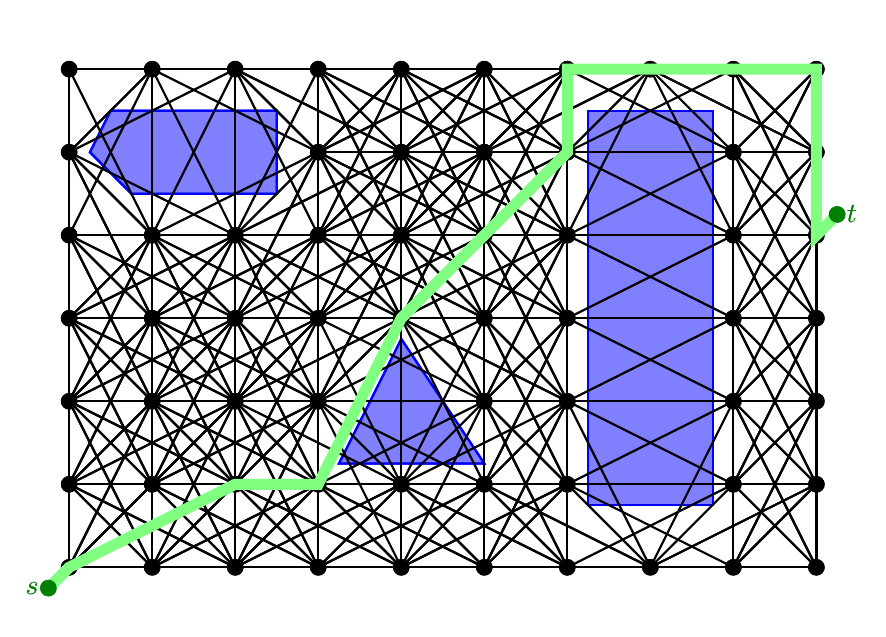
\begin{tikzpicture}[x=15pt,y=15pt]
\path [use as bounding box,red] (0,0) rectangle (20,14);
\fill[green!50!black](0.5,0.5) node[left]{\(s\)}circle (3pt);
\fill[green!50!black](19.5,9.5) node[right]{\(t\)}circle (3pt);
\fill<2>(1,1)circle (3pt);
\fill<2>(1,3)circle (3pt);
\fill<2>(1,5)circle (3pt);
\fill<2>(1,7)circle (3pt);
\fill<2>(1,9)circle (3pt);
\fill<2>(1,11)circle (3pt);
\fill<2>(1,13)circle (3pt);
\fill<2>(3,1)circle (3pt);
\fill<2>(3,3)circle (3pt);
\fill<2>(3,5)circle (3pt);
\fill<2>(3,7)circle (3pt);
\fill<2>(3,9)circle (3pt);
\fill<2>(3,11)circle (3pt);
\fill<2>(3,13)circle (3pt);
\fill<2>(5,1)circle (3pt);
\fill<2>(5,3)circle (3pt);
\fill<2>(5,5)circle (3pt);
\fill<2>(5,7)circle (3pt);
\fill<2>(5,9)circle (3pt);
\fill<2>(5,11)circle (3pt);
\fill<2>(5,13)circle (3pt);
\fill<2>(7,1)circle (3pt);
\fill<2>(7,3)circle (3pt);
\fill<2>(7,5)circle (3pt);
\fill<2>(7,7)circle (3pt);
\fill<2>(7,9)circle (3pt);
\fill<2>(7,11)circle (3pt);
\fill<2>(7,13)circle (3pt);
\fill<2>(9,1)circle (3pt);
\fill<2>(9,3)circle (3pt);
\fill<2>(9,5)circle (3pt);
\fill<2>(9,7)circle (3pt);
\fill<2>(9,9)circle (3pt);
\fill<2>(9,11)circle (3pt);
\fill<2>(9,13)circle (3pt);
\fill<2>(11,1)circle (3pt);
\fill<2>(11,3)circle (3pt);
\fill<2>(11,5)circle (3pt);
\fill<2>(11,7)circle (3pt);
\fill<2>(11,9)circle (3pt);
\fill<2>(11,11)circle (3pt);
\fill<2>(11,13)circle (3pt);
\fill<2>(13,1)circle (3pt);
\fill<2>(13,3)circle (3pt);
\fill<2>(13,5)circle (3pt);
\fill<2>(13,7)circle (3pt);
\fill<2>(13,9)circle (3pt);
\fill<2>(13,11)circle (3pt);
\fill<2>(13,13)circle (3pt);
\fill<2>(15,1)circle (3pt);
\fill<2>(15,3)circle (3pt);
\fill<2>(15,5)circle (3pt);
\fill<2>(15,7)circle (3pt);
\fill<2>(15,9)circle (3pt);
\fill<2>(15,11)circle (3pt);
\fill<2>(15,13)circle (3pt);
\fill<2>(17,1)circle (3pt);
\fill<2>(17,3)circle (3pt);
\fill<2>(17,5)circle (3pt);
\fill<2>(17,7)circle (3pt);
\fill<2>(17,9)circle (3pt);
\fill<2>(17,11)circle (3pt);
\fill<2>(17,13)circle (3pt);
\fill<2>(19,1)circle (3pt);
\fill<2>(19,3)circle (3pt);
\fill<2>(19,5)circle (3pt);
\fill<2>(19,7)circle (3pt);
\fill<2>(19,9)circle (3pt);
\fill<2>(19,11)circle (3pt);
\fill<2>(19,13)circle (3pt);
\fill<3-7>(1,1)circle (3pt);
\fill<3-7>(1,3)circle (3pt);
\fill<3-7>(1,5)circle (3pt);
\fill<3-7>(1,7)circle (3pt);
\fill<3-7>(1,9)circle (3pt);
\fill<3-7>(1,11)circle (3pt);
\fill<3-7>(1,13)circle (3pt);
\fill<3-7>(3,1)circle (3pt);
\fill<3-7>(3,3)circle (3pt);
\fill<3-7>(3,5)circle (3pt);
\fill<3-7>(3,7)circle (3pt);
\fill<3-7>(3,9)circle (3pt);
\fill<3-7>(3,13)circle (3pt);
\fill<3-7>(5,1)circle (3pt);
\fill<3-7>(5,3)circle (3pt);
\fill<3-7>(5,5)circle (3pt);
\fill<3-7>(5,7)circle (3pt);
\fill<3-7>(5,9)circle (3pt);
\fill<3-7>(5,13)circle (3pt);
\fill<3-7>(7,1)circle (3pt);
\fill<3-7>(7,3)circle (3pt);
\fill<3-7>(7,5)circle (3pt);
\fill<3-7>(7,7)circle (3pt);
\fill<3-7>(7,9)circle (3pt);
\fill<3-7>(7,11)circle (3pt);
\fill<3-7>(7,13)circle (3pt);
\fill<3-7>(9,1)circle (3pt);
\fill<3-7>(9,3)circle (3pt);
\fill<3-7>(9,7)circle (3pt);
\fill<3-7>(9,9)circle (3pt);
\fill<3-7>(9,11)circle (3pt);
\fill<3-7>(9,13)circle (3pt);
\fill<3-7>(11,1)circle (3pt);
\fill<3-7>(11,3)circle (3pt);
\fill<3-7>(11,5)circle (3pt);
\fill<3-7>(11,7)circle (3pt);
\fill<3-7>(11,9)circle (3pt);
\fill<3-7>(11,11)circle (3pt);
\fill<3-7>(11,13)circle (3pt);
\fill<3-7>(13,1)circle (3pt);
\fill<3-7>(13,3)circle (3pt);
\fill<3-7>(13,5)circle (3pt);
\fill<3-7>(13,7)circle (3pt);
\fill<3-7>(13,9)circle (3pt);
\fill<3-7>(13,11)circle (3pt);
\fill<3-7>(13,13)circle (3pt);
\fill<3-7>(15,1)circle (3pt);
\fill<3-7>(15,13)circle (3pt);
\fill<3-7>(17,1)circle (3pt);
\fill<3-7>(17,3)circle (3pt);
\fill<3-7>(17,5)circle (3pt);
\fill<3-7>(17,7)circle (3pt);
\fill<3-7>(17,9)circle (3pt);
\fill<3-7>(17,11)circle (3pt);
\fill<3-7>(17,13)circle (3pt);
\fill<3-7>(19,1)circle (3pt);
\fill<3-7>(19,3)circle (3pt);
\fill<3-7>(19,5)circle (3pt);
\fill<3-7>(19,7)circle (3pt);
\fill<3-7>(19,9)circle (3pt);
\fill<3-7>(19,11)circle (3pt);
\fill<3-7>(19,13)circle (3pt);
\draw<1,3->[thick,blue,fill=blue!50] (7.5,3.5) -- (11,3.5) -- (9,6.5) -- cycle;
\draw<2>[thick,blue,fill=blue!50,fill opacity=0.5] (7.5,3.5) -- (11,3.5) -- (9,6.5) -- cycle;
\draw<1,3->[thick,blue,fill=blue!50] (2.5,10) -- (6,10) -- (6,12) -- (2,12) -- (1.5,11) -- cycle;
\draw<2>[thick,blue,fill=blue!50,fill opacity=0.5] (2.5,10) -- (6,10) -- (6,12) -- (2,12) -- (1.5,11) -- cycle;
\draw<1,3->[thick,blue,fill=blue!50] (13.5,2.5) -- (16.5,2.5) -- (16.5,12) -- (13.5,12) -- cycle;
\draw<2>[thick,blue,fill=blue!50,fill opacity=0.5] (13.5,2.5) -- (16.5,2.5) -- (16.5,12) -- (13.5,12) -- cycle;
\draw<4>[thick](1,1) -- (1,3);
\draw<4>[thick](1,1) -- (1,5);
\draw<4>[thick](1,1) -- (3,1);
\draw<4>[thick](1,1) -- (3,3);
\draw<4>[thick](1,1) -- (3,5);
\draw<4>[thick](1,1) -- (5,1);
\draw<4>[thick](1,1) -- (5,3);
\draw<4>[thick](1,3) -- (1,5);
\draw<4>[thick](1,3) -- (1,7);
\draw<4>[thick](1,3) -- (3,1);
\draw<4>[thick](1,3) -- (3,3);
\draw<4>[thick](1,3) -- (3,5);
\draw<4>[thick](1,3) -- (3,7);
\draw<4>[thick](1,3) -- (5,1);
\draw<4>[thick](1,3) -- (5,3);
\draw<4>[thick](1,3) -- (5,5);
\draw<4>[thick](1,5) -- (1,7);
\draw<4>[thick](1,5) -- (1,9);
\draw<4>[thick](1,5) -- (3,1);
\draw<4>[thick](1,5) -- (3,3);
\draw<4>[thick](1,5) -- (3,5);
\draw<4>[thick](1,5) -- (3,7);
\draw<4>[thick](1,5) -- (3,9);
\draw<4>[thick](1,5) -- (5,3);
\draw<4>[thick](1,5) -- (5,5);
\draw<4>[thick](1,5) -- (5,7);
\draw<4>[thick](1,7) -- (1,9);
\draw<4>[thick](1,7) -- (1,11);
\draw<4>[thick](1,7) -- (3,3);
\draw<4>[thick](1,7) -- (3,5);
\draw<4>[thick](1,7) -- (3,7);
\draw<4>[thick](1,7) -- (3,9);
\draw<4>[thick](1,7) -- (5,5);
\draw<4>[thick](1,7) -- (5,7);
\draw<4>[thick](1,7) -- (5,9);
\draw<4>[thick](1,9) -- (1,11);
\draw<4>[thick](1,9) -- (1,13);
\draw<4>[thick](1,9) -- (3,5);
\draw<4>[thick](1,9) -- (3,7);
\draw<4>[thick](1,9) -- (3,9);
\draw<4>[thick](1,9) -- (3,13);
\draw<4>[thick](1,9) -- (5,7);
\draw<4>[thick](1,9) -- (5,9);
\draw<4>[thick](1,11) -- (1,13);
\draw<4>[thick](1,11) -- (3,7);
\draw<4>[thick](1,11) -- (3,9);
\draw<4>[thick](1,11) -- (3,13);
\draw<4>[thick](1,11) -- (5,9);
\draw<4>[thick](1,11) -- (5,13);
\draw<4>[thick](1,13) -- (3,9);
\draw<4>[thick](1,13) -- (3,13);
\draw<4>[thick](1,13) -- (5,13);
\draw<4>[thick](3,1) -- (3,3);
\draw<4>[thick](3,1) -- (3,5);
\draw<4>[thick](3,1) -- (5,1);
\draw<4>[thick](3,1) -- (5,3);
\draw<4>[thick](3,1) -- (5,5);
\draw<4>[thick](3,1) -- (7,1);
\draw<4>[thick](3,1) -- (7,3);
\draw<4>[thick](3,3) -- (3,5);
\draw<4>[thick](3,3) -- (3,7);
\draw<4>[thick](3,3) -- (5,1);
\draw<4>[thick](3,3) -- (5,3);
\draw<4>[thick](3,3) -- (5,5);
\draw<4>[thick](3,3) -- (5,7);
\draw<4>[thick](3,3) -- (7,1);
\draw<4>[thick](3,3) -- (7,3);
\draw<4>[thick](3,3) -- (7,5);
\draw<4>[thick](3,5) -- (3,7);
\draw<4>[thick](3,5) -- (3,9);
\draw<4>[thick](3,5) -- (5,1);
\draw<4>[thick](3,5) -- (5,3);
\draw<4>[thick](3,5) -- (5,5);
\draw<4>[thick](3,5) -- (5,7);
\draw<4>[thick](3,5) -- (5,9);
\draw<4>[thick](3,5) -- (7,3);
\draw<4>[thick](3,5) -- (7,5);
\draw<4>[thick](3,5) -- (7,7);
\draw<4>[thick](3,7) -- (3,9);
\draw<4>[thick](3,7) -- (5,3);
\draw<4>[thick](3,7) -- (5,5);
\draw<4>[thick](3,7) -- (5,7);
\draw<4>[thick](3,7) -- (5,9);
\draw<4>[thick](3,7) -- (7,5);
\draw<4>[thick](3,7) -- (7,7);
\draw<4>[thick](3,7) -- (7,9);
\draw<4>[thick](3,9) -- (3,13);
\draw<4>[thick](3,9) -- (5,5);
\draw<4>[thick](3,9) -- (5,7);
\draw<4>[thick](3,9) -- (5,9);
\draw<4>[thick](3,9) -- (5,13);
\draw<4>[thick](3,9) -- (7,7);
\draw<4>[thick](3,9) -- (7,9);
\draw<4>[thick](3,9) -- (7,11);
\draw<4>[thick](3,13) -- (5,9);
\draw<4>[thick](3,13) -- (5,13);
\draw<4>[thick](3,13) -- (7,11);
\draw<4>[thick](3,13) -- (7,13);
\draw<4>[thick](5,1) -- (5,3);
\draw<4>[thick](5,1) -- (5,5);
\draw<4>[thick](5,1) -- (7,1);
\draw<4>[thick](5,1) -- (7,3);
\draw<4>[thick](5,1) -- (7,5);
\draw<4>[thick](5,1) -- (9,1);
\draw<4>[thick](5,1) -- (9,3);
\draw<4>[thick](5,3) -- (5,5);
\draw<4>[thick](5,3) -- (5,7);
\draw<4>[thick](5,3) -- (7,1);
\draw<4>[thick](5,3) -- (7,3);
\draw<4>[thick](5,3) -- (7,5);
\draw<4>[thick](5,3) -- (7,7);
\draw<4>[thick](5,3) -- (9,1);
\draw<4>[thick](5,3) -- (9,3);
\draw<4>[thick](5,5) -- (5,7);
\draw<4>[thick](5,5) -- (5,9);
\draw<4>[thick](5,5) -- (7,1);
\draw<4>[thick](5,5) -- (7,3);
\draw<4>[thick](5,5) -- (7,5);
\draw<4>[thick](5,5) -- (7,7);
\draw<4>[thick](5,5) -- (7,9);
\draw<4>[thick](5,5) -- (9,3);
\draw<4>[thick](5,5) -- (9,7);
\draw<4>[thick](5,7) -- (5,9);
\draw<4>[thick](5,7) -- (7,3);
\draw<4>[thick](5,7) -- (7,5);
\draw<4>[thick](5,7) -- (7,7);
\draw<4>[thick](5,7) -- (7,9);
\draw<4>[thick](5,7) -- (7,11);
\draw<4>[thick](5,7) -- (9,7);
\draw<4>[thick](5,7) -- (9,9);
\draw<4>[thick](5,9) -- (5,13);
\draw<4>[thick](5,9) -- (7,5);
\draw<4>[thick](5,9) -- (7,7);
\draw<4>[thick](5,9) -- (7,9);
\draw<4>[thick](5,9) -- (7,11);
\draw<4>[thick](5,9) -- (7,13);
\draw<4>[thick](5,9) -- (9,7);
\draw<4>[thick](5,9) -- (9,9);
\draw<4>[thick](5,9) -- (9,11);
\draw<4>[thick](5,13) -- (7,9);
\draw<4>[thick](5,13) -- (7,11);
\draw<4>[thick](5,13) -- (7,13);
\draw<4>[thick](5,13) -- (9,11);
\draw<4>[thick](5,13) -- (9,13);
\draw<4>[thick](7,1) -- (7,3);
\draw<4>[thick](7,1) -- (7,5);
\draw<4>[thick](7,1) -- (9,1);
\draw<4>[thick](7,1) -- (9,3);
\draw<4>[thick](7,1) -- (11,1);
\draw<4>[thick](7,1) -- (11,3);
\draw<4>[thick](7,3) -- (7,5);
\draw<4>[thick](7,3) -- (7,7);
\draw<4>[thick](7,3) -- (9,1);
\draw<4>[thick](7,3) -- (9,3);
\draw<4>[thick](7,3) -- (9,7);
\draw<4>[thick](7,3) -- (11,1);
\draw<4>[thick](7,3) -- (11,3);
\draw<4>[thick](7,3) -- (11,5);
\draw<4>[thick](7,5) -- (7,7);
\draw<4>[thick](7,5) -- (7,9);
\draw<4>[thick](7,5) -- (9,1);
\draw<4>[thick](7,5) -- (9,3);
\draw<4>[thick](7,5) -- (9,7);
\draw<4>[thick](7,5) -- (9,9);
\draw<4>[thick](7,5) -- (11,3);
\draw<4>[thick](7,5) -- (11,5);
\draw<4>[thick](7,5) -- (11,7);
\draw<4>[thick](7,7) -- (7,9);
\draw<4>[thick](7,7) -- (7,11);
\draw<4>[thick](7,7) -- (9,3);
\draw<4>[thick](7,7) -- (9,7);
\draw<4>[thick](7,7) -- (9,9);
\draw<4>[thick](7,7) -- (9,11);
\draw<4>[thick](7,7) -- (11,5);
\draw<4>[thick](7,7) -- (11,7);
\draw<4>[thick](7,7) -- (11,9);
\draw<4>[thick](7,9) -- (7,11);
\draw<4>[thick](7,9) -- (7,13);
\draw<4>[thick](7,9) -- (9,7);
\draw<4>[thick](7,9) -- (9,9);
\draw<4>[thick](7,9) -- (9,11);
\draw<4>[thick](7,9) -- (9,13);
\draw<4>[thick](7,9) -- (11,7);
\draw<4>[thick](7,9) -- (11,9);
\draw<4>[thick](7,9) -- (11,11);
\draw<4>[thick](7,11) -- (7,13);
\draw<4>[thick](7,11) -- (9,7);
\draw<4>[thick](7,11) -- (9,9);
\draw<4>[thick](7,11) -- (9,11);
\draw<4>[thick](7,11) -- (9,13);
\draw<4>[thick](7,11) -- (11,9);
\draw<4>[thick](7,11) -- (11,11);
\draw<4>[thick](7,11) -- (11,13);
\draw<4>[thick](7,13) -- (9,9);
\draw<4>[thick](7,13) -- (9,11);
\draw<4>[thick](7,13) -- (9,13);
\draw<4>[thick](7,13) -- (11,11);
\draw<4>[thick](7,13) -- (11,13);
\draw<4>[thick](9,1) -- (9,3);
\draw<4>[thick](9,1) -- (11,1);
\draw<4>[thick](9,1) -- (11,3);
\draw<4>[thick](9,1) -- (11,5);
\draw<4>[thick](9,1) -- (13,1);
\draw<4>[thick](9,1) -- (13,3);
\draw<4>[thick](9,3) -- (9,7);
\draw<4>[thick](9,3) -- (11,1);
\draw<4>[thick](9,3) -- (11,3);
\draw<4>[thick](9,3) -- (11,5);
\draw<4>[thick](9,3) -- (11,7);
\draw<4>[thick](9,3) -- (13,1);
\draw<4>[thick](9,3) -- (13,3);
\draw<4>[thick](9,3) -- (13,5);
\draw<4>[thick](9,7) -- (9,9);
\draw<4>[thick](9,7) -- (9,11);
\draw<4>[thick](9,7) -- (11,3);
\draw<4>[thick](9,7) -- (11,5);
\draw<4>[thick](9,7) -- (11,7);
\draw<4>[thick](9,7) -- (11,9);
\draw<4>[thick](9,7) -- (11,11);
\draw<4>[thick](9,7) -- (13,5);
\draw<4>[thick](9,7) -- (13,7);
\draw<4>[thick](9,7) -- (13,9);
\draw<4>[thick](9,9) -- (9,11);
\draw<4>[thick](9,9) -- (9,13);
\draw<4>[thick](9,9) -- (11,5);
\draw<4>[thick](9,9) -- (11,7);
\draw<4>[thick](9,9) -- (11,9);
\draw<4>[thick](9,9) -- (11,11);
\draw<4>[thick](9,9) -- (11,13);
\draw<4>[thick](9,9) -- (13,7);
\draw<4>[thick](9,9) -- (13,9);
\draw<4>[thick](9,9) -- (13,11);
\draw<4>[thick](9,11) -- (9,13);
\draw<4>[thick](9,11) -- (11,7);
\draw<4>[thick](9,11) -- (11,9);
\draw<4>[thick](9,11) -- (11,11);
\draw<4>[thick](9,11) -- (11,13);
\draw<4>[thick](9,11) -- (13,9);
\draw<4>[thick](9,11) -- (13,11);
\draw<4>[thick](9,11) -- (13,13);
\draw<4>[thick](9,13) -- (11,9);
\draw<4>[thick](9,13) -- (11,11);
\draw<4>[thick](9,13) -- (11,13);
\draw<4>[thick](9,13) -- (13,11);
\draw<4>[thick](9,13) -- (13,13);
\draw<4>[thick](11,1) -- (11,3);
\draw<4>[thick](11,1) -- (11,5);
\draw<4>[thick](11,1) -- (13,1);
\draw<4>[thick](11,1) -- (13,3);
\draw<4>[thick](11,1) -- (13,5);
\draw<4>[thick](11,1) -- (15,1);
\draw<4>[thick](11,3) -- (11,5);
\draw<4>[thick](11,3) -- (11,7);
\draw<4>[thick](11,3) -- (13,1);
\draw<4>[thick](11,3) -- (13,3);
\draw<4>[thick](11,3) -- (13,5);
\draw<4>[thick](11,3) -- (13,7);
\draw<4>[thick](11,3) -- (15,1);
\draw<4>[thick](11,5) -- (11,7);
\draw<4>[thick](11,5) -- (11,9);
\draw<4>[thick](11,5) -- (13,1);
\draw<4>[thick](11,5) -- (13,3);
\draw<4>[thick](11,5) -- (13,5);
\draw<4>[thick](11,5) -- (13,7);
\draw<4>[thick](11,5) -- (13,9);
\draw<4>[thick](11,7) -- (11,9);
\draw<4>[thick](11,7) -- (11,11);
\draw<4>[thick](11,7) -- (13,3);
\draw<4>[thick](11,7) -- (13,5);
\draw<4>[thick](11,7) -- (13,7);
\draw<4>[thick](11,7) -- (13,9);
\draw<4>[thick](11,7) -- (13,11);
\draw<4>[thick](11,9) -- (11,11);
\draw<4>[thick](11,9) -- (11,13);
\draw<4>[thick](11,9) -- (13,5);
\draw<4>[thick](11,9) -- (13,7);
\draw<4>[thick](11,9) -- (13,9);
\draw<4>[thick](11,9) -- (13,11);
\draw<4>[thick](11,9) -- (13,13);
\draw<4>[thick](11,11) -- (11,13);
\draw<4>[thick](11,11) -- (13,7);
\draw<4>[thick](11,11) -- (13,9);
\draw<4>[thick](11,11) -- (13,11);
\draw<4>[thick](11,11) -- (13,13);
\draw<4>[thick](11,11) -- (15,13);
\draw<4>[thick](11,13) -- (13,9);
\draw<4>[thick](11,13) -- (13,11);
\draw<4>[thick](11,13) -- (13,13);
\draw<4>[thick](11,13) -- (15,13);
\draw<4>[thick](13,1) -- (13,3);
\draw<4>[thick](13,1) -- (13,5);
\draw<4>[thick](13,1) -- (15,1);
\draw<4>[thick](13,1) -- (17,1);
\draw<4>[thick](13,1) -- (17,3);
\draw<4>[thick](13,3) -- (13,5);
\draw<4>[thick](13,3) -- (13,7);
\draw<4>[thick](13,3) -- (15,1);
\draw<4>[thick](13,3) -- (17,1);
\draw<4>[thick](13,3) -- (17,3);
\draw<4>[thick](13,3) -- (17,5);
\draw<4>[thick](13,5) -- (13,7);
\draw<4>[thick](13,5) -- (13,9);
\draw<4>[thick](13,5) -- (15,1);
\draw<4>[thick](13,5) -- (17,3);
\draw<4>[thick](13,5) -- (17,5);
\draw<4>[thick](13,5) -- (17,7);
\draw<4>[thick](13,7) -- (13,9);
\draw<4>[thick](13,7) -- (13,11);
\draw<4>[thick](13,7) -- (17,5);
\draw<4>[thick](13,7) -- (17,7);
\draw<4>[thick](13,7) -- (17,9);
\draw<4>[thick](13,9) -- (13,11);
\draw<4>[thick](13,9) -- (13,13);
\draw<4>[thick](13,9) -- (15,13);
\draw<4>[thick](13,9) -- (17,7);
\draw<4>[thick](13,9) -- (17,9);
\draw<4>[thick](13,9) -- (17,11);
\draw<4>[thick](13,11) -- (13,13);
\draw<4>[thick](13,11) -- (15,13);
\draw<4>[thick](13,11) -- (17,9);
\draw<4>[thick](13,11) -- (17,11);
\draw<4>[thick](13,11) -- (17,13);
\draw<4>[thick](13,13) -- (15,13);
\draw<4>[thick](13,13) -- (17,11);
\draw<4>[thick](13,13) -- (17,13);
\draw<4>[thick](15,1) -- (17,1);
\draw<4>[thick](15,1) -- (17,3);
\draw<4>[thick](15,1) -- (17,5);
\draw<4>[thick](15,1) -- (19,1);
\draw<4>[thick](15,1) -- (19,3);
\draw<4>[thick](15,13) -- (17,9);
\draw<4>[thick](15,13) -- (17,11);
\draw<4>[thick](15,13) -- (17,13);
\draw<4>[thick](15,13) -- (19,11);
\draw<4>[thick](15,13) -- (19,13);
\draw<4>[thick](17,1) -- (17,3);
\draw<4>[thick](17,1) -- (17,5);
\draw<4>[thick](17,1) -- (19,1);
\draw<4>[thick](17,1) -- (19,3);
\draw<4>[thick](17,1) -- (19,5);
\draw<4>[thick](17,3) -- (17,5);
\draw<4>[thick](17,3) -- (17,7);
\draw<4>[thick](17,3) -- (19,1);
\draw<4>[thick](17,3) -- (19,3);
\draw<4>[thick](17,3) -- (19,5);
\draw<4>[thick](17,3) -- (19,7);
\draw<4>[thick](17,5) -- (17,7);
\draw<4>[thick](17,5) -- (17,9);
\draw<4>[thick](17,5) -- (19,1);
\draw<4>[thick](17,5) -- (19,3);
\draw<4>[thick](17,5) -- (19,5);
\draw<4>[thick](17,5) -- (19,7);
\draw<4>[thick](17,5) -- (19,9);
\draw<4>[thick](17,7) -- (17,9);
\draw<4>[thick](17,7) -- (17,11);
\draw<4>[thick](17,7) -- (19,3);
\draw<4>[thick](17,7) -- (19,5);
\draw<4>[thick](17,7) -- (19,7);
\draw<4>[thick](17,7) -- (19,9);
\draw<4>[thick](17,7) -- (19,11);
\draw<4>[thick](17,9) -- (17,11);
\draw<4>[thick](17,9) -- (17,13);
\draw<4>[thick](17,9) -- (19,5);
\draw<4>[thick](17,9) -- (19,7);
\draw<4>[thick](17,9) -- (19,9);
\draw<4>[thick](17,9) -- (19,11);
\draw<4>[thick](17,9) -- (19,13);
\draw<4>[thick](17,11) -- (17,13);
\draw<4>[thick](17,11) -- (19,7);
\draw<4>[thick](17,11) -- (19,9);
\draw<4>[thick](17,11) -- (19,11);
\draw<4>[thick](17,11) -- (19,13);
\draw<4>[thick](17,13) -- (19,9);
\draw<4>[thick](17,13) -- (19,11);
\draw<4>[thick](17,13) -- (19,13);
\draw<4>[thick](19,1) -- (19,3);
\draw<4>[thick](19,1) -- (19,5);
\draw<4>[thick](19,3) -- (19,5);
\draw<4>[thick](19,3) -- (19,7);
\draw<4>[thick](19,5) -- (19,7);
\draw<4>[thick](19,5) -- (19,9);
\draw<4>[thick](19,7) -- (19,9);
\draw<4>[thick](19,7) -- (19,11);
\draw<4>[thick](19,9) -- (19,11);
\draw<4>[thick](19,9) -- (19,13);
\draw<4>[thick](19,11) -- (19,13);
\draw<5-7>[thick](1,1) -- (1,3);
\draw<5-7>[thick](1,1) -- (1,5);
\draw<5-7>[thick](1,1) -- (3,1);
\draw<5-7>[thick](1,1) -- (3,3);
\draw<5-7>[thick](1,1) -- (3,5);
\draw<5-7>[thick](1,1) -- (5,1);
\draw<5-7>[thick](1,1) -- (5,3);
\draw<5-7>[thick](1,3) -- (1,5);
\draw<5-7>[thick](1,3) -- (1,7);
\draw<5-7>[thick](1,3) -- (3,1);
\draw<5-7>[thick](1,3) -- (3,3);
\draw<5-7>[thick](1,3) -- (3,5);
\draw<5-7>[thick](1,3) -- (3,7);
\draw<5-7>[thick](1,3) -- (5,1);
\draw<5-7>[thick](1,3) -- (5,3);
\draw<5-7>[thick](1,3) -- (5,5);
\draw<5-7>[thick](1,5) -- (1,7);
\draw<5-7>[thick](1,5) -- (1,9);
\draw<5-7>[thick](1,5) -- (3,1);
\draw<5-7>[thick](1,5) -- (3,3);
\draw<5-7>[thick](1,5) -- (3,5);
\draw<5-7>[thick](1,5) -- (3,7);
\draw<5-7>[thick](1,5) -- (3,9);
\draw<5-7>[thick](1,5) -- (5,3);
\draw<5-7>[thick](1,5) -- (5,5);
\draw<5-7>[thick](1,5) -- (5,7);
\draw<5-7>[thick](1,7) -- (1,9);
\draw<5-7>[thick](1,7) -- (1,11);
\draw<5-7>[thick](1,7) -- (3,3);
\draw<5-7>[thick](1,7) -- (3,5);
\draw<5-7>[thick](1,7) -- (3,7);
\draw<5-7>[thick](1,7) -- (3,9);
\draw<5-7>[thick](1,7) -- (5,5);
\draw<5-7>[thick](1,7) -- (5,7);
\draw<5-7>[thick](1,7) -- (5,9);
\draw<5-7>[thick](1,9) -- (1,11);
\draw<5-7>[thick](1,9) -- (1,13);
\draw<5-7>[thick](1,9) -- (3,5);
\draw<5-7>[thick](1,9) -- (3,7);
\draw<5-7>[thick](1,9) -- (3,9);
\draw<5-7>[thick](1,9) -- (5,7);
\draw<5-7>[thick](1,9) -- (5,9);
\draw<5-7>[thick](1,11) -- (1,13);
\draw<5-7>[thick](1,11) -- (3,7);
\draw<5-7>[thick](1,11) -- (3,9);
\draw<5-7>[thick](1,11) -- (3,13);
\draw<5-7>[thick](1,13) -- (3,13);
\draw<5-7>[thick](1,13) -- (5,13);
\draw<5-7>[thick](3,1) -- (3,3);
\draw<5-7>[thick](3,1) -- (3,5);
\draw<5-7>[thick](3,1) -- (5,1);
\draw<5-7>[thick](3,1) -- (5,3);
\draw<5-7>[thick](3,1) -- (5,5);
\draw<5-7>[thick](3,1) -- (7,1);
\draw<5-7>[thick](3,1) -- (7,3);
\draw<5-7>[thick](3,3) -- (3,5);
\draw<5-7>[thick](3,3) -- (3,7);
\draw<5-7>[thick](3,3) -- (5,1);
\draw<5-7>[thick](3,3) -- (5,3);
\draw<5-7>[thick](3,3) -- (5,5);
\draw<5-7>[thick](3,3) -- (5,7);
\draw<5-7>[thick](3,3) -- (7,1);
\draw<5-7>[thick](3,3) -- (7,3);
\draw<5-7>[thick](3,3) -- (7,5);
\draw<5-7>[thick](3,5) -- (3,7);
\draw<5-7>[thick](3,5) -- (3,9);
\draw<5-7>[thick](3,5) -- (5,1);
\draw<5-7>[thick](3,5) -- (5,3);
\draw<5-7>[thick](3,5) -- (5,5);
\draw<5-7>[thick](3,5) -- (5,7);
\draw<5-7>[thick](3,5) -- (5,9);
\draw<5-7>[thick](3,5) -- (7,3);
\draw<5-7>[thick](3,5) -- (7,5);
\draw<5-7>[thick](3,5) -- (7,7);
\draw<5-7>[thick](3,7) -- (3,9);
\draw<5-7>[thick](3,7) -- (5,3);
\draw<5-7>[thick](3,7) -- (5,5);
\draw<5-7>[thick](3,7) -- (5,7);
\draw<5-7>[thick](3,7) -- (5,9);
\draw<5-7>[thick](3,7) -- (7,5);
\draw<5-7>[thick](3,7) -- (7,7);
\draw<5-7>[thick](3,7) -- (7,9);
\draw<5-7>[thick](3,9) -- (5,5);
\draw<5-7>[thick](3,9) -- (5,7);
\draw<5-7>[thick](3,9) -- (5,9);
\draw<5-7>[thick](3,9) -- (7,7);
\draw<5-7>[thick](3,9) -- (7,9);
\draw<5-7>[thick](3,13) -- (5,13);
\draw<5-7>[thick](3,13) -- (7,13);
\draw<5-7>[thick](5,1) -- (5,3);
\draw<5-7>[thick](5,1) -- (5,5);
\draw<5-7>[thick](5,1) -- (7,1);
\draw<5-7>[thick](5,1) -- (7,3);
\draw<5-7>[thick](5,1) -- (7,5);
\draw<5-7>[thick](5,1) -- (9,1);
\draw<5-7>[thick](5,1) -- (9,3);
\draw<5-7>[thick](5,3) -- (5,5);
\draw<5-7>[thick](5,3) -- (5,7);
\draw<5-7>[thick](5,3) -- (7,1);
\draw<5-7>[thick](5,3) -- (7,3);
\draw<5-7>[thick](5,3) -- (7,5);
\draw<5-7>[thick](5,3) -- (7,7);
\draw<5-7>[thick](5,3) -- (9,1);
\draw<5-7>[thick](5,3) -- (9,3);
\draw<5-7>[thick](5,5) -- (5,7);
\draw<5-7>[thick](5,5) -- (5,9);
\draw<5-7>[thick](5,5) -- (7,1);
\draw<5-7>[thick](5,5) -- (7,3);
\draw<5-7>[thick](5,5) -- (7,5);
\draw<5-7>[thick](5,5) -- (7,7);
\draw<5-7>[thick](5,5) -- (7,9);
\draw<5-7>[thick](5,5) -- (9,7);
\draw<5-7>[thick](5,7) -- (5,9);
\draw<5-7>[thick](5,7) -- (7,3);
\draw<5-7>[thick](5,7) -- (7,5);
\draw<5-7>[thick](5,7) -- (7,7);
\draw<5-7>[thick](5,7) -- (7,9);
\draw<5-7>[thick](5,7) -- (7,11);
\draw<5-7>[thick](5,7) -- (9,7);
\draw<5-7>[thick](5,7) -- (9,9);
\draw<5-7>[thick](5,9) -- (7,5);
\draw<5-7>[thick](5,9) -- (7,7);
\draw<5-7>[thick](5,9) -- (7,9);
\draw<5-7>[thick](5,9) -- (9,7);
\draw<5-7>[thick](5,9) -- (9,9);
\draw<5-7>[thick](5,9) -- (9,11);
\draw<5-7>[thick](5,13) -- (7,11);
\draw<5-7>[thick](5,13) -- (7,13);
\draw<5-7>[thick](5,13) -- (9,11);
\draw<5-7>[thick](5,13) -- (9,13);
\draw<5-7>[thick](7,1) -- (7,3);
\draw<5-7>[thick](7,1) -- (7,5);
\draw<5-7>[thick](7,1) -- (9,1);
\draw<5-7>[thick](7,1) -- (9,3);
\draw<5-7>[thick](7,1) -- (11,1);
\draw<5-7>[thick](7,1) -- (11,3);
\draw<5-7>[thick](7,3) -- (7,5);
\draw<5-7>[thick](7,3) -- (7,7);
\draw<5-7>[thick](7,3) -- (9,1);
\draw<5-7>[thick](7,3) -- (9,3);
\draw<5-7>[thick](7,3) -- (9,7);
\draw<5-7>[thick](7,3) -- (11,1);
\draw<5-7>[thick](7,3) -- (11,3);
\draw<5-7>[thick](7,5) -- (7,7);
\draw<5-7>[thick](7,5) -- (7,9);
\draw<5-7>[thick](7,5) -- (9,7);
\draw<5-7>[thick](7,5) -- (9,9);
\draw<5-7>[thick](7,7) -- (7,9);
\draw<5-7>[thick](7,7) -- (7,11);
\draw<5-7>[thick](7,7) -- (9,7);
\draw<5-7>[thick](7,7) -- (9,9);
\draw<5-7>[thick](7,7) -- (9,11);
\draw<5-7>[thick](7,7) -- (11,7);
\draw<5-7>[thick](7,7) -- (11,9);
\draw<5-7>[thick](7,9) -- (7,11);
\draw<5-7>[thick](7,9) -- (7,13);
\draw<5-7>[thick](7,9) -- (9,7);
\draw<5-7>[thick](7,9) -- (9,9);
\draw<5-7>[thick](7,9) -- (9,11);
\draw<5-7>[thick](7,9) -- (9,13);
\draw<5-7>[thick](7,9) -- (11,7);
\draw<5-7>[thick](7,9) -- (11,9);
\draw<5-7>[thick](7,9) -- (11,11);
\draw<5-7>[thick](7,11) -- (7,13);
\draw<5-7>[thick](7,11) -- (9,7);
\draw<5-7>[thick](7,11) -- (9,9);
\draw<5-7>[thick](7,11) -- (9,11);
\draw<5-7>[thick](7,11) -- (9,13);
\draw<5-7>[thick](7,11) -- (11,9);
\draw<5-7>[thick](7,11) -- (11,11);
\draw<5-7>[thick](7,11) -- (11,13);
\draw<5-7>[thick](7,13) -- (9,9);
\draw<5-7>[thick](7,13) -- (9,11);
\draw<5-7>[thick](7,13) -- (9,13);
\draw<5-7>[thick](7,13) -- (11,11);
\draw<5-7>[thick](7,13) -- (11,13);
\draw<5-7>[thick](9,1) -- (9,3);
\draw<5-7>[thick](9,1) -- (11,1);
\draw<5-7>[thick](9,1) -- (11,3);
\draw<5-7>[thick](9,1) -- (13,1);
\draw<5-7>[thick](9,1) -- (13,3);
\draw<5-7>[thick](9,3) -- (11,1);
\draw<5-7>[thick](9,3) -- (11,3);
\draw<5-7>[thick](9,3) -- (13,1);
\draw<5-7>[thick](9,3) -- (13,3);
\draw<5-7>[thick](9,7) -- (9,9);
\draw<5-7>[thick](9,7) -- (9,11);
\draw<5-7>[thick](9,7) -- (11,5);
\draw<5-7>[thick](9,7) -- (11,7);
\draw<5-7>[thick](9,7) -- (11,9);
\draw<5-7>[thick](9,7) -- (11,11);
\draw<5-7>[thick](9,7) -- (13,5);
\draw<5-7>[thick](9,7) -- (13,7);
\draw<5-7>[thick](9,7) -- (13,9);
\draw<5-7>[thick](9,9) -- (9,11);
\draw<5-7>[thick](9,9) -- (9,13);
\draw<5-7>[thick](9,9) -- (11,5);
\draw<5-7>[thick](9,9) -- (11,7);
\draw<5-7>[thick](9,9) -- (11,9);
\draw<5-7>[thick](9,9) -- (11,11);
\draw<5-7>[thick](9,9) -- (11,13);
\draw<5-7>[thick](9,9) -- (13,7);
\draw<5-7>[thick](9,9) -- (13,9);
\draw<5-7>[thick](9,9) -- (13,11);
\draw<5-7>[thick](9,11) -- (9,13);
\draw<5-7>[thick](9,11) -- (11,7);
\draw<5-7>[thick](9,11) -- (11,9);
\draw<5-7>[thick](9,11) -- (11,11);
\draw<5-7>[thick](9,11) -- (11,13);
\draw<5-7>[thick](9,11) -- (13,9);
\draw<5-7>[thick](9,11) -- (13,11);
\draw<5-7>[thick](9,11) -- (13,13);
\draw<5-7>[thick](9,13) -- (11,9);
\draw<5-7>[thick](9,13) -- (11,11);
\draw<5-7>[thick](9,13) -- (11,13);
\draw<5-7>[thick](9,13) -- (13,11);
\draw<5-7>[thick](9,13) -- (13,13);
\draw<5-7>[thick](11,1) -- (11,3);
\draw<5-7>[thick](11,1) -- (13,1);
\draw<5-7>[thick](11,1) -- (13,3);
\draw<5-7>[thick](11,1) -- (13,5);
\draw<5-7>[thick](11,1) -- (15,1);
\draw<5-7>[thick](11,3) -- (13,1);
\draw<5-7>[thick](11,3) -- (13,3);
\draw<5-7>[thick](11,3) -- (13,5);
\draw<5-7>[thick](11,3) -- (13,7);
\draw<5-7>[thick](11,3) -- (15,1);
\draw<5-7>[thick](11,5) -- (11,7);
\draw<5-7>[thick](11,5) -- (11,9);
\draw<5-7>[thick](11,5) -- (13,1);
\draw<5-7>[thick](11,5) -- (13,3);
\draw<5-7>[thick](11,5) -- (13,5);
\draw<5-7>[thick](11,5) -- (13,7);
\draw<5-7>[thick](11,5) -- (13,9);
\draw<5-7>[thick](11,7) -- (11,9);
\draw<5-7>[thick](11,7) -- (11,11);
\draw<5-7>[thick](11,7) -- (13,3);
\draw<5-7>[thick](11,7) -- (13,5);
\draw<5-7>[thick](11,7) -- (13,7);
\draw<5-7>[thick](11,7) -- (13,9);
\draw<5-7>[thick](11,7) -- (13,11);
\draw<5-7>[thick](11,9) -- (11,11);
\draw<5-7>[thick](11,9) -- (11,13);
\draw<5-7>[thick](11,9) -- (13,5);
\draw<5-7>[thick](11,9) -- (13,7);
\draw<5-7>[thick](11,9) -- (13,9);
\draw<5-7>[thick](11,9) -- (13,11);
\draw<5-7>[thick](11,9) -- (13,13);
\draw<5-7>[thick](11,11) -- (11,13);
\draw<5-7>[thick](11,11) -- (13,7);
\draw<5-7>[thick](11,11) -- (13,9);
\draw<5-7>[thick](11,11) -- (13,11);
\draw<5-7>[thick](11,11) -- (13,13);
\draw<5-7>[thick](11,11) -- (15,13);
\draw<5-7>[thick](11,13) -- (13,9);
\draw<5-7>[thick](11,13) -- (13,11);
\draw<5-7>[thick](11,13) -- (13,13);
\draw<5-7>[thick](11,13) -- (15,13);
\draw<5-7>[thick](13,1) -- (13,3);
\draw<5-7>[thick](13,1) -- (13,5);
\draw<5-7>[thick](13,1) -- (15,1);
\draw<5-7>[thick](13,1) -- (17,1);
\draw<5-7>[thick](13,3) -- (13,5);
\draw<5-7>[thick](13,3) -- (13,7);
\draw<5-7>[thick](13,5) -- (13,7);
\draw<5-7>[thick](13,5) -- (13,9);
\draw<5-7>[thick](13,7) -- (13,9);
\draw<5-7>[thick](13,7) -- (13,11);
\draw<5-7>[thick](13,9) -- (13,11);
\draw<5-7>[thick](13,9) -- (13,13);
\draw<5-7>[thick](13,11) -- (13,13);
\draw<5-7>[thick](13,13) -- (15,13);
\draw<5-7>[thick](13,13) -- (17,13);
\draw<5-7>[thick](15,1) -- (17,1);
\draw<5-7>[thick](15,1) -- (19,1);
\draw<5-7>[thick](15,1) -- (19,3);
\draw<5-7>[thick](15,13) -- (17,13);
\draw<5-7>[thick](15,13) -- (19,11);
\draw<5-7>[thick](15,13) -- (19,13);
\draw<5-7>[thick](17,1) -- (17,3);
\draw<5-7>[thick](17,1) -- (17,5);
\draw<5-7>[thick](17,1) -- (19,1);
\draw<5-7>[thick](17,1) -- (19,3);
\draw<5-7>[thick](17,1) -- (19,5);
\draw<5-7>[thick](17,3) -- (17,5);
\draw<5-7>[thick](17,3) -- (17,7);
\draw<5-7>[thick](17,3) -- (19,1);
\draw<5-7>[thick](17,3) -- (19,3);
\draw<5-7>[thick](17,3) -- (19,5);
\draw<5-7>[thick](17,3) -- (19,7);
\draw<5-7>[thick](17,5) -- (17,7);
\draw<5-7>[thick](17,5) -- (17,9);
\draw<5-7>[thick](17,5) -- (19,1);
\draw<5-7>[thick](17,5) -- (19,3);
\draw<5-7>[thick](17,5) -- (19,5);
\draw<5-7>[thick](17,5) -- (19,7);
\draw<5-7>[thick](17,5) -- (19,9);
\draw<5-7>[thick](17,7) -- (17,9);
\draw<5-7>[thick](17,7) -- (17,11);
\draw<5-7>[thick](17,7) -- (19,3);
\draw<5-7>[thick](17,7) -- (19,5);
\draw<5-7>[thick](17,7) -- (19,7);
\draw<5-7>[thick](17,7) -- (19,9);
\draw<5-7>[thick](17,7) -- (19,11);
\draw<5-7>[thick](17,9) -- (17,11);
\draw<5-7>[thick](17,9) -- (17,13);
\draw<5-7>[thick](17,9) -- (19,5);
\draw<5-7>[thick](17,9) -- (19,7);
\draw<5-7>[thick](17,9) -- (19,9);
\draw<5-7>[thick](17,9) -- (19,11);
\draw<5-7>[thick](17,9) -- (19,13);
\draw<5-7>[thick](17,11) -- (17,13);
\draw<5-7>[thick](17,11) -- (19,7);
\draw<5-7>[thick](17,11) -- (19,9);
\draw<5-7>[thick](17,11) -- (19,11);
\draw<5-7>[thick](17,11) -- (19,13);
\draw<5-7>[thick](17,13) -- (19,9);
\draw<5-7>[thick](17,13) -- (19,11);
\draw<5-7>[thick](17,13) -- (19,13);
\draw<5-7>[thick](19,1) -- (19,3);
\draw<5-7>[thick](19,1) -- (19,5);
\draw<5-7>[thick](19,3) -- (19,5);
\draw<5-7>[thick](19,3) -- (19,7);
\draw<5-7>[thick](19,5) -- (19,7);
\draw<5-7>[thick](19,5) -- (19,9);
\draw<5-7>[thick](19,7) -- (19,9);
\draw<5-7>[thick](19,7) -- (19,11);
\draw<5-7>[thick](19,9) -- (19,11);
\draw<5-7>[thick](19,9) -- (19,13);
\draw<5-7>[thick](19,11) -- (19,13);
\draw<6-8>[line width = 4pt,green!50,line cap=round] (0.5,0.5)-- (1,1)(19,9) -- (19.5,9.5);
\draw<7-8>[line width = 4pt,green!50] (0.5,0.5) -- (1,1) -- (5,3) -- (7,3) -- (9,7) -- (13,11) -- (13,13) -- (19,13) -- (19,9) -- (19.5,9.5);
\fill<6-8>[green!50!black](0.5,0.5) node[left]{\(s\)}circle (3pt);
\fill<6-8>[green!50!black](19.5,9.5) node[right]{\(t\)}circle (3pt);
\end{tikzpicture}

  \end{center}
\end{frame}

\begin{frame}<1-2>[label=prm-impl-details]
  \frametitle{Classical PRM \headingCite{Ka96}}
  \vspace{-1.5ex}
  \onslide<+->{
  \begin{algorithm}[H]
    \begin{algorithmic}[1]
      \STATE \(V \leftarrow \emptyset\) ; \(E \leftarrow \emptyset\)
      \LOOP
        \alert<2,3,4>{\STATE \(\cp{q} \leftarrow\) a point in \(\cfree\)}
        \STATE \(V \leftarrow V \cup \{\cp{q}\}\)
        \alert<2>{\STATE \(N_{\cp{q}} \leftarrow\) useful neighbors of \(\cp{q}\)}
        \FORALL{\(\cp{q}' \in N_{\cp{q}}\)}
          \IF{\(\cp{q}'\) and \(\cp{q}\) are not connected in \(\mathcal{G}\)}
            \IF{the \alert<2,5>{local planner} finds a path between \(\cp{q}'\) and \(\cp{q}\)}
              \STATE \(E \leftarrow E \cup \overline{\cp{q}\cp{q}'}\)
            \ENDIF
          \ENDIF
        \ENDFOR
      \ENDLOOP
    \end{algorithmic}
    \caption{PRMBuildGraph}
  \end{algorithm}
  \vspace{-2ex}
  }
  \begin{block}<3->{PRM Implementation Details}
    \begin{itemize}
    \item<3-|alert@3> {How to sample?}
    \item<4-|alert@4> {Determine whether a sample point is free?}
    \item<5-|alert@5> {How to determine whether an \emph{edge} is free or not?}
    \end{itemize}
  \end{block}
\end{frame}

\subsection*{Sampling}

\againframe<3>{prm-impl-details}

\begin{frame}
  \frametitle{Sample the Configuration Space}
  \begin{alertblock}{Objective}
    Obtain a (uniform) sample of \cfree{}
  \end{alertblock}
  \begin{block}{Steps}
    \begin{itemize}
    \item (Randomly) pick \(\cp{q} \in \cspace\)
    \item \emph{Collision detection} for \(\robot(\cp{q})\)
    \end{itemize}
  \end{block}
  \note{
    \begin{itemize}
    \item Uniform: more important the sample has to be dense in the problematic regions of the cspace.
    \end{itemize}
  }
\end{frame}

\begin{frame}[allowframebreaks,label=main-cspace-pts-pick]
  \frametitle{Configuration Points Picking}
  \begin{itemize}
  \item Random
  \item Grid
  \item Cell-Based
  \item Halton points (pseudo random and deterministic!)~\hyperlink{app-halton}{\beamerbutton{more\dots}}
  \item Random-Halton
  \end{itemize}
\end{frame}

\subsection*{Collision Detection}

\againframe<4>{prm-impl-details}

\begin{frame}
  \frametitle{Collision Detection}
  \begin{definition}[Predicate]
    \begin{center}
      \(\phi \colon \cspace \to \{\mathrm{TRUE,FALSE}\}\), s.t.:%
    \end{center}
    \[%
    \phi(\cp{q}) =
    \begin{cases}
      \mathrm{TRUE} & \text{if } \cp{q} \in \cforb\\
      \mathrm{FALSE} & \text{otherwise}
    \end{cases}
    \]%
  \end{definition}

  \begin{definition}[Distance Function]
    The distance in \wspace{} between \(\robot(\cp{q})\) and the obstacles is measured by \(d \colon \cspace \to [0,\infty)\).
  \end{definition}
  \note{
    \begin{itemize}
    \item If \(d(\cp{q})=0\), then \(\phi(\cp{q}) = TRUE\)
    \end{itemize}
  }
\end{frame}

\begin{frame}
  \frametitle{Two-phase Collision Detection}
  \begin{alertblock}{Fact}
    Collision detection is an expensive task that is repeatedly invoked!
  \end{alertblock}
  %
  \begin{block}{Break-up the Task}
    \begin{itemize}
    \item Broad Phase (e.g. using bounding boxes)
    \item Narrow Phase (e.g. using hierarchical methods; See~\cite[\S~5.3.2]{La06})
    \end{itemize}
  \end{block}
\end{frame}

\subsection*{Local Planner}
\againframe<5>{prm-impl-details}

\begin{frame}
  \frametitle{Local Planner}

  \begin{block}{Objective}
    Given \(\cp{q},\cp{q}' \in \cfree\) find a path in \cfree{} connecting them.
  \end{block}

  \begin{block}{Trade-off}
    \begin{itemize}
    \item Accurate and slow
    \item\alert<2->{Inaccurate and quick}
    \end{itemize}
  \end{block}
\end{frame}

\begin{frame}
  \frametitle{General Local Planner \headingCite{Ka96}}
  \begin{block}{}
    \begin{itemize}
    \item Given \(\cp{q},\cp{q}' \in \cfree\)
    \item Let \(\{\cp{c}_i\}\) be points on the \emph{line} connecting \(\cp{q}\) and \(\cp{q}'\), s.t. \(\mathrm{d}(\robot(\cp{c}_i),\robot(\cp{c}_{i+1})) \leq \epsilon\)
    \item \(\forall i\): collision detection for \(\robot_\epsilon(\cp{c}_i)\)
    \end{itemize}
  \end{block}
\end{frame}

\begin{frame}
  \frametitle{Binary Local Planner \headingCite{Ro02}}
  \begin{block}{}
    \begin{itemize}
    \item Given \(\cp{q},\cp{q}' \in \cfree\)
    \item Let \(\cp{c}\) be the midpoint of the \emph{line} connecting \(\cp{q}\) and \(\cp{q}'\)
      \begin{itemize}
      \item Collision detection for \(\robot(\cp{c})\)
      \item Repeat on two sides of \(\cp{c}\)
      \end{itemize}
    \end{itemize}
  \end{block}
\end{frame}

\subsection*{Completeness of the Method}

\begin{frame}
  \frametitle{Completeness of the Method}
  \begin{definition}<2->
    A method is \emph{probabilistically complete} if the probability of answering a query \emph{incorrectly} after building a roadmap tends to zero as the number of samples goes to \emph{infinity}.
  \end{definition}
\end{frame}

\begin{frame}
  \frametitle{Influencing Parameters}
  \begin{itemize}
  \item \(N\) - number of samples
  \item \(\gamma \colon [0,L] \to \cfree\) - free path from \(\gamma(0) = \cp{s}\) to \(\gamma(L) = \cp{t}\).
  \item \(R = \inf_{0 \leq t \leq L} \inf_{y \in\obst}|\gamma(t) - y|\)
  \end{itemize}

  \begin{theorem}[\cite{Ka98}]
  %
  \[%
  P(\fail) \leq \frac{2L}{R} \left( 1 - \frac{\pi R^2}{4 |\cfree|} \right)^N
  \]%
\end{theorem}
%%% Local Variables:
%%% mode: latex
%%% TeX-master: "defense-motion-planning"
%%% End:

\end{frame}

\begin{frame}
  \frametitle{PRM is Probabilistic Complete}
  \begin{theorem}[\cite{Ka98}]
  %
  \[%
  P(\fail) \leq \frac{2L}{R} \left( 1 - \frac{\pi R^2}{4 |\cfree|} \right)^N
  \]%
\end{theorem}
%%% Local Variables:
%%% mode: latex
%%% TeX-master: "defense-motion-planning"
%%% End:

  \begin{columns}
    \only<1-4>{
    \begin{column}{0.46\textwidth}
      \begin{itemize}
      \item<2-4> \(n = \ceil{2L/R}\) points on \(\gamma\)
      \item<2-4> \(d(\cp{x}_i,\cp{x}_{i+1}) \leq R/2\) and \(B_{R/2}(\cp{x}_{i+1}) \subset B_R(\cp{x}_i)\)
      \item<3-4> \(\Rightarrow \overline{\cp{c}\cp{d}}\) is free
      \item<4> PRM succeeds if each \(B_{R/2}(\cp{x}_j)\) contains a sample
      \item<4> \(P(B_{R/2}(\cp{x}_j) \text{ is empty}) = \left(1-\frac{|B_{R/2}|}{|\cfree|}\right)^N\)
      \end{itemize}
    \end{column}
  }
\only<5->{
  \begin{column}{0.46\textwidth}
    \begin{align*}
      & P(\fail)\\
      & \leq P(\text{some ball is empty}) \\
      & \leq \sum_{j=1}^{n-1} P(j\text{-th ball is empty})\\
      & = \left( \ceil[\Bigg]{\frac{2L}{R}}-1 \right) \left( 1- \frac{|B_{R/2}|}{|\cfree|} \right)^N
    \end{align*}
  \end{column}
}
    \begin{column}{0.54\textwidth}
      \begin{center}
        \begin{tikzpicture}
  \def\ptRad{3pt}
  \def\rRad{2.5}
  \coordinate (a) at (-3,-1);
  \coordinate (b) at (3,1);

  \draw<1->[ultra thick,%
        insert node={\node[red](xtmp){};} at 0.47,
        insert node={\node[red](xitmp){};} at 0.65
  ] plot [smooth,tension=.95] %
  coordinates{(a) (-1,0) (0,0) (1,0) (b)};
  \coordinate (x) at (xtmp.center);
  \coordinate (xi) at (xitmp.center);

  \fill<1-> (a) node[below=2*\ptRad]{\(\cp{s}\)} circle (\ptRad);
  \fill<1-> (b) node[above=2*\ptRad]{\(\cp{t}\)} circle (\ptRad);
  \fill<2-> (x) circle (\ptRad);
  \fill<2-> (xi) circle (\ptRad);

  \onslide<2->{
  \draw[dashed] (x) circle (\rRad);
  \draw (x) node[below left]{\(\cp{x}_i\)} -- +(130:\rRad) node[sloped,above,pos=0.65]{\(R\)};
  \draw (xi) node[below right]{\(\cp{x}_{i+1}\)} -- +(65:0.5*\rRad) node[sloped,below,pos=0.65]{\(\frac{R}{2}\)};
  \draw (x) circle (0.5*\rRad);
  \draw (xi) circle (0.5*\rRad);
}

\onslide<3->{
  \coordinate (c) at ($(x)+(250:0.5*\rRad)$);
  \coordinate (d) at ($(xi)+(275:0.5*\rRad)$);
  \draw[thick,blue] (c) -- (d);
  \fill (c) node[below left]{\(\cp{c}\)} circle (\ptRad);
  \fill (d) node[below right]{\(\cp{d}\)} circle (\ptRad);
}
\end{tikzpicture}
%%% Local Variables:
%%% mode: latex
%%% TeX-master: "../defense-motion-planning"
%%% End:

      \end{center}
    \end{column}
  \end{columns}
\end{frame}

\subsection*{Summary}
\againframe{prm-overview}

\section[MMS]{Motion Planning via Manifold Samples (\cite{Sa13})}
\begin{frame}<5>
  \frametitle{Motion Planning via Manifold Samples \headingCite{Sa13}}
  \begin{itemize}
  \item In PRM connectivity of \cspace{} is captured via point samples
  \item Try to obtain ``bigger'' samples and improve the capturing
  \end{itemize}
  \begin{center}
    \scalebox{0.7}{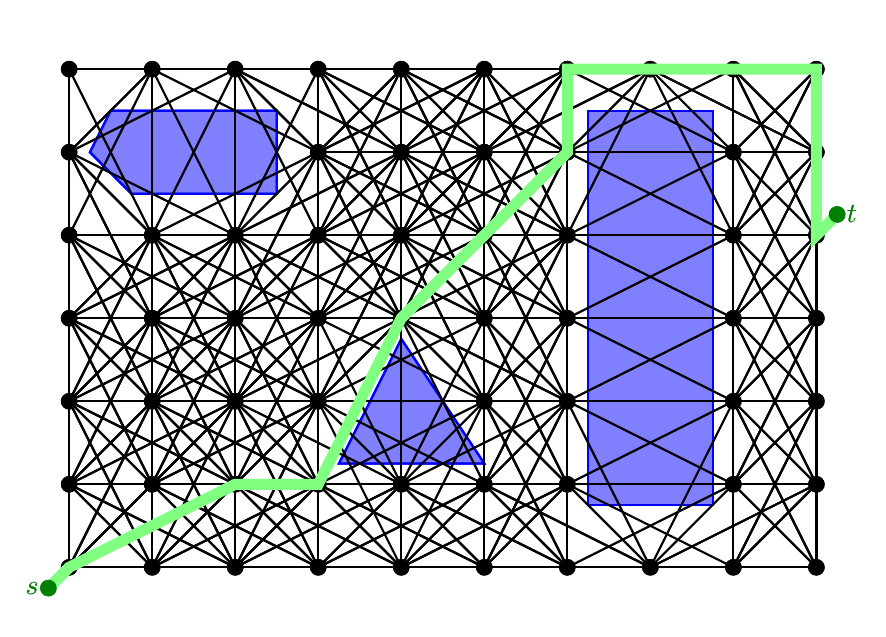
\begin{tikzpicture}[x=15pt,y=15pt]
\path [use as bounding box,red] (0,0) rectangle (20,14);
\fill[green!50!black](0.5,0.5) node[left]{\(s\)}circle (3pt);
\fill[green!50!black](19.5,9.5) node[right]{\(t\)}circle (3pt);
\fill<2>(1,1)circle (3pt);
\fill<2>(1,3)circle (3pt);
\fill<2>(1,5)circle (3pt);
\fill<2>(1,7)circle (3pt);
\fill<2>(1,9)circle (3pt);
\fill<2>(1,11)circle (3pt);
\fill<2>(1,13)circle (3pt);
\fill<2>(3,1)circle (3pt);
\fill<2>(3,3)circle (3pt);
\fill<2>(3,5)circle (3pt);
\fill<2>(3,7)circle (3pt);
\fill<2>(3,9)circle (3pt);
\fill<2>(3,11)circle (3pt);
\fill<2>(3,13)circle (3pt);
\fill<2>(5,1)circle (3pt);
\fill<2>(5,3)circle (3pt);
\fill<2>(5,5)circle (3pt);
\fill<2>(5,7)circle (3pt);
\fill<2>(5,9)circle (3pt);
\fill<2>(5,11)circle (3pt);
\fill<2>(5,13)circle (3pt);
\fill<2>(7,1)circle (3pt);
\fill<2>(7,3)circle (3pt);
\fill<2>(7,5)circle (3pt);
\fill<2>(7,7)circle (3pt);
\fill<2>(7,9)circle (3pt);
\fill<2>(7,11)circle (3pt);
\fill<2>(7,13)circle (3pt);
\fill<2>(9,1)circle (3pt);
\fill<2>(9,3)circle (3pt);
\fill<2>(9,5)circle (3pt);
\fill<2>(9,7)circle (3pt);
\fill<2>(9,9)circle (3pt);
\fill<2>(9,11)circle (3pt);
\fill<2>(9,13)circle (3pt);
\fill<2>(11,1)circle (3pt);
\fill<2>(11,3)circle (3pt);
\fill<2>(11,5)circle (3pt);
\fill<2>(11,7)circle (3pt);
\fill<2>(11,9)circle (3pt);
\fill<2>(11,11)circle (3pt);
\fill<2>(11,13)circle (3pt);
\fill<2>(13,1)circle (3pt);
\fill<2>(13,3)circle (3pt);
\fill<2>(13,5)circle (3pt);
\fill<2>(13,7)circle (3pt);
\fill<2>(13,9)circle (3pt);
\fill<2>(13,11)circle (3pt);
\fill<2>(13,13)circle (3pt);
\fill<2>(15,1)circle (3pt);
\fill<2>(15,3)circle (3pt);
\fill<2>(15,5)circle (3pt);
\fill<2>(15,7)circle (3pt);
\fill<2>(15,9)circle (3pt);
\fill<2>(15,11)circle (3pt);
\fill<2>(15,13)circle (3pt);
\fill<2>(17,1)circle (3pt);
\fill<2>(17,3)circle (3pt);
\fill<2>(17,5)circle (3pt);
\fill<2>(17,7)circle (3pt);
\fill<2>(17,9)circle (3pt);
\fill<2>(17,11)circle (3pt);
\fill<2>(17,13)circle (3pt);
\fill<2>(19,1)circle (3pt);
\fill<2>(19,3)circle (3pt);
\fill<2>(19,5)circle (3pt);
\fill<2>(19,7)circle (3pt);
\fill<2>(19,9)circle (3pt);
\fill<2>(19,11)circle (3pt);
\fill<2>(19,13)circle (3pt);
\fill<3-7>(1,1)circle (3pt);
\fill<3-7>(1,3)circle (3pt);
\fill<3-7>(1,5)circle (3pt);
\fill<3-7>(1,7)circle (3pt);
\fill<3-7>(1,9)circle (3pt);
\fill<3-7>(1,11)circle (3pt);
\fill<3-7>(1,13)circle (3pt);
\fill<3-7>(3,1)circle (3pt);
\fill<3-7>(3,3)circle (3pt);
\fill<3-7>(3,5)circle (3pt);
\fill<3-7>(3,7)circle (3pt);
\fill<3-7>(3,9)circle (3pt);
\fill<3-7>(3,13)circle (3pt);
\fill<3-7>(5,1)circle (3pt);
\fill<3-7>(5,3)circle (3pt);
\fill<3-7>(5,5)circle (3pt);
\fill<3-7>(5,7)circle (3pt);
\fill<3-7>(5,9)circle (3pt);
\fill<3-7>(5,13)circle (3pt);
\fill<3-7>(7,1)circle (3pt);
\fill<3-7>(7,3)circle (3pt);
\fill<3-7>(7,5)circle (3pt);
\fill<3-7>(7,7)circle (3pt);
\fill<3-7>(7,9)circle (3pt);
\fill<3-7>(7,11)circle (3pt);
\fill<3-7>(7,13)circle (3pt);
\fill<3-7>(9,1)circle (3pt);
\fill<3-7>(9,3)circle (3pt);
\fill<3-7>(9,7)circle (3pt);
\fill<3-7>(9,9)circle (3pt);
\fill<3-7>(9,11)circle (3pt);
\fill<3-7>(9,13)circle (3pt);
\fill<3-7>(11,1)circle (3pt);
\fill<3-7>(11,3)circle (3pt);
\fill<3-7>(11,5)circle (3pt);
\fill<3-7>(11,7)circle (3pt);
\fill<3-7>(11,9)circle (3pt);
\fill<3-7>(11,11)circle (3pt);
\fill<3-7>(11,13)circle (3pt);
\fill<3-7>(13,1)circle (3pt);
\fill<3-7>(13,3)circle (3pt);
\fill<3-7>(13,5)circle (3pt);
\fill<3-7>(13,7)circle (3pt);
\fill<3-7>(13,9)circle (3pt);
\fill<3-7>(13,11)circle (3pt);
\fill<3-7>(13,13)circle (3pt);
\fill<3-7>(15,1)circle (3pt);
\fill<3-7>(15,13)circle (3pt);
\fill<3-7>(17,1)circle (3pt);
\fill<3-7>(17,3)circle (3pt);
\fill<3-7>(17,5)circle (3pt);
\fill<3-7>(17,7)circle (3pt);
\fill<3-7>(17,9)circle (3pt);
\fill<3-7>(17,11)circle (3pt);
\fill<3-7>(17,13)circle (3pt);
\fill<3-7>(19,1)circle (3pt);
\fill<3-7>(19,3)circle (3pt);
\fill<3-7>(19,5)circle (3pt);
\fill<3-7>(19,7)circle (3pt);
\fill<3-7>(19,9)circle (3pt);
\fill<3-7>(19,11)circle (3pt);
\fill<3-7>(19,13)circle (3pt);
\draw<1,3->[thick,blue,fill=blue!50] (7.5,3.5) -- (11,3.5) -- (9,6.5) -- cycle;
\draw<2>[thick,blue,fill=blue!50,fill opacity=0.5] (7.5,3.5) -- (11,3.5) -- (9,6.5) -- cycle;
\draw<1,3->[thick,blue,fill=blue!50] (2.5,10) -- (6,10) -- (6,12) -- (2,12) -- (1.5,11) -- cycle;
\draw<2>[thick,blue,fill=blue!50,fill opacity=0.5] (2.5,10) -- (6,10) -- (6,12) -- (2,12) -- (1.5,11) -- cycle;
\draw<1,3->[thick,blue,fill=blue!50] (13.5,2.5) -- (16.5,2.5) -- (16.5,12) -- (13.5,12) -- cycle;
\draw<2>[thick,blue,fill=blue!50,fill opacity=0.5] (13.5,2.5) -- (16.5,2.5) -- (16.5,12) -- (13.5,12) -- cycle;
\draw<4>[thick](1,1) -- (1,3);
\draw<4>[thick](1,1) -- (1,5);
\draw<4>[thick](1,1) -- (3,1);
\draw<4>[thick](1,1) -- (3,3);
\draw<4>[thick](1,1) -- (3,5);
\draw<4>[thick](1,1) -- (5,1);
\draw<4>[thick](1,1) -- (5,3);
\draw<4>[thick](1,3) -- (1,5);
\draw<4>[thick](1,3) -- (1,7);
\draw<4>[thick](1,3) -- (3,1);
\draw<4>[thick](1,3) -- (3,3);
\draw<4>[thick](1,3) -- (3,5);
\draw<4>[thick](1,3) -- (3,7);
\draw<4>[thick](1,3) -- (5,1);
\draw<4>[thick](1,3) -- (5,3);
\draw<4>[thick](1,3) -- (5,5);
\draw<4>[thick](1,5) -- (1,7);
\draw<4>[thick](1,5) -- (1,9);
\draw<4>[thick](1,5) -- (3,1);
\draw<4>[thick](1,5) -- (3,3);
\draw<4>[thick](1,5) -- (3,5);
\draw<4>[thick](1,5) -- (3,7);
\draw<4>[thick](1,5) -- (3,9);
\draw<4>[thick](1,5) -- (5,3);
\draw<4>[thick](1,5) -- (5,5);
\draw<4>[thick](1,5) -- (5,7);
\draw<4>[thick](1,7) -- (1,9);
\draw<4>[thick](1,7) -- (1,11);
\draw<4>[thick](1,7) -- (3,3);
\draw<4>[thick](1,7) -- (3,5);
\draw<4>[thick](1,7) -- (3,7);
\draw<4>[thick](1,7) -- (3,9);
\draw<4>[thick](1,7) -- (5,5);
\draw<4>[thick](1,7) -- (5,7);
\draw<4>[thick](1,7) -- (5,9);
\draw<4>[thick](1,9) -- (1,11);
\draw<4>[thick](1,9) -- (1,13);
\draw<4>[thick](1,9) -- (3,5);
\draw<4>[thick](1,9) -- (3,7);
\draw<4>[thick](1,9) -- (3,9);
\draw<4>[thick](1,9) -- (3,13);
\draw<4>[thick](1,9) -- (5,7);
\draw<4>[thick](1,9) -- (5,9);
\draw<4>[thick](1,11) -- (1,13);
\draw<4>[thick](1,11) -- (3,7);
\draw<4>[thick](1,11) -- (3,9);
\draw<4>[thick](1,11) -- (3,13);
\draw<4>[thick](1,11) -- (5,9);
\draw<4>[thick](1,11) -- (5,13);
\draw<4>[thick](1,13) -- (3,9);
\draw<4>[thick](1,13) -- (3,13);
\draw<4>[thick](1,13) -- (5,13);
\draw<4>[thick](3,1) -- (3,3);
\draw<4>[thick](3,1) -- (3,5);
\draw<4>[thick](3,1) -- (5,1);
\draw<4>[thick](3,1) -- (5,3);
\draw<4>[thick](3,1) -- (5,5);
\draw<4>[thick](3,1) -- (7,1);
\draw<4>[thick](3,1) -- (7,3);
\draw<4>[thick](3,3) -- (3,5);
\draw<4>[thick](3,3) -- (3,7);
\draw<4>[thick](3,3) -- (5,1);
\draw<4>[thick](3,3) -- (5,3);
\draw<4>[thick](3,3) -- (5,5);
\draw<4>[thick](3,3) -- (5,7);
\draw<4>[thick](3,3) -- (7,1);
\draw<4>[thick](3,3) -- (7,3);
\draw<4>[thick](3,3) -- (7,5);
\draw<4>[thick](3,5) -- (3,7);
\draw<4>[thick](3,5) -- (3,9);
\draw<4>[thick](3,5) -- (5,1);
\draw<4>[thick](3,5) -- (5,3);
\draw<4>[thick](3,5) -- (5,5);
\draw<4>[thick](3,5) -- (5,7);
\draw<4>[thick](3,5) -- (5,9);
\draw<4>[thick](3,5) -- (7,3);
\draw<4>[thick](3,5) -- (7,5);
\draw<4>[thick](3,5) -- (7,7);
\draw<4>[thick](3,7) -- (3,9);
\draw<4>[thick](3,7) -- (5,3);
\draw<4>[thick](3,7) -- (5,5);
\draw<4>[thick](3,7) -- (5,7);
\draw<4>[thick](3,7) -- (5,9);
\draw<4>[thick](3,7) -- (7,5);
\draw<4>[thick](3,7) -- (7,7);
\draw<4>[thick](3,7) -- (7,9);
\draw<4>[thick](3,9) -- (3,13);
\draw<4>[thick](3,9) -- (5,5);
\draw<4>[thick](3,9) -- (5,7);
\draw<4>[thick](3,9) -- (5,9);
\draw<4>[thick](3,9) -- (5,13);
\draw<4>[thick](3,9) -- (7,7);
\draw<4>[thick](3,9) -- (7,9);
\draw<4>[thick](3,9) -- (7,11);
\draw<4>[thick](3,13) -- (5,9);
\draw<4>[thick](3,13) -- (5,13);
\draw<4>[thick](3,13) -- (7,11);
\draw<4>[thick](3,13) -- (7,13);
\draw<4>[thick](5,1) -- (5,3);
\draw<4>[thick](5,1) -- (5,5);
\draw<4>[thick](5,1) -- (7,1);
\draw<4>[thick](5,1) -- (7,3);
\draw<4>[thick](5,1) -- (7,5);
\draw<4>[thick](5,1) -- (9,1);
\draw<4>[thick](5,1) -- (9,3);
\draw<4>[thick](5,3) -- (5,5);
\draw<4>[thick](5,3) -- (5,7);
\draw<4>[thick](5,3) -- (7,1);
\draw<4>[thick](5,3) -- (7,3);
\draw<4>[thick](5,3) -- (7,5);
\draw<4>[thick](5,3) -- (7,7);
\draw<4>[thick](5,3) -- (9,1);
\draw<4>[thick](5,3) -- (9,3);
\draw<4>[thick](5,5) -- (5,7);
\draw<4>[thick](5,5) -- (5,9);
\draw<4>[thick](5,5) -- (7,1);
\draw<4>[thick](5,5) -- (7,3);
\draw<4>[thick](5,5) -- (7,5);
\draw<4>[thick](5,5) -- (7,7);
\draw<4>[thick](5,5) -- (7,9);
\draw<4>[thick](5,5) -- (9,3);
\draw<4>[thick](5,5) -- (9,7);
\draw<4>[thick](5,7) -- (5,9);
\draw<4>[thick](5,7) -- (7,3);
\draw<4>[thick](5,7) -- (7,5);
\draw<4>[thick](5,7) -- (7,7);
\draw<4>[thick](5,7) -- (7,9);
\draw<4>[thick](5,7) -- (7,11);
\draw<4>[thick](5,7) -- (9,7);
\draw<4>[thick](5,7) -- (9,9);
\draw<4>[thick](5,9) -- (5,13);
\draw<4>[thick](5,9) -- (7,5);
\draw<4>[thick](5,9) -- (7,7);
\draw<4>[thick](5,9) -- (7,9);
\draw<4>[thick](5,9) -- (7,11);
\draw<4>[thick](5,9) -- (7,13);
\draw<4>[thick](5,9) -- (9,7);
\draw<4>[thick](5,9) -- (9,9);
\draw<4>[thick](5,9) -- (9,11);
\draw<4>[thick](5,13) -- (7,9);
\draw<4>[thick](5,13) -- (7,11);
\draw<4>[thick](5,13) -- (7,13);
\draw<4>[thick](5,13) -- (9,11);
\draw<4>[thick](5,13) -- (9,13);
\draw<4>[thick](7,1) -- (7,3);
\draw<4>[thick](7,1) -- (7,5);
\draw<4>[thick](7,1) -- (9,1);
\draw<4>[thick](7,1) -- (9,3);
\draw<4>[thick](7,1) -- (11,1);
\draw<4>[thick](7,1) -- (11,3);
\draw<4>[thick](7,3) -- (7,5);
\draw<4>[thick](7,3) -- (7,7);
\draw<4>[thick](7,3) -- (9,1);
\draw<4>[thick](7,3) -- (9,3);
\draw<4>[thick](7,3) -- (9,7);
\draw<4>[thick](7,3) -- (11,1);
\draw<4>[thick](7,3) -- (11,3);
\draw<4>[thick](7,3) -- (11,5);
\draw<4>[thick](7,5) -- (7,7);
\draw<4>[thick](7,5) -- (7,9);
\draw<4>[thick](7,5) -- (9,1);
\draw<4>[thick](7,5) -- (9,3);
\draw<4>[thick](7,5) -- (9,7);
\draw<4>[thick](7,5) -- (9,9);
\draw<4>[thick](7,5) -- (11,3);
\draw<4>[thick](7,5) -- (11,5);
\draw<4>[thick](7,5) -- (11,7);
\draw<4>[thick](7,7) -- (7,9);
\draw<4>[thick](7,7) -- (7,11);
\draw<4>[thick](7,7) -- (9,3);
\draw<4>[thick](7,7) -- (9,7);
\draw<4>[thick](7,7) -- (9,9);
\draw<4>[thick](7,7) -- (9,11);
\draw<4>[thick](7,7) -- (11,5);
\draw<4>[thick](7,7) -- (11,7);
\draw<4>[thick](7,7) -- (11,9);
\draw<4>[thick](7,9) -- (7,11);
\draw<4>[thick](7,9) -- (7,13);
\draw<4>[thick](7,9) -- (9,7);
\draw<4>[thick](7,9) -- (9,9);
\draw<4>[thick](7,9) -- (9,11);
\draw<4>[thick](7,9) -- (9,13);
\draw<4>[thick](7,9) -- (11,7);
\draw<4>[thick](7,9) -- (11,9);
\draw<4>[thick](7,9) -- (11,11);
\draw<4>[thick](7,11) -- (7,13);
\draw<4>[thick](7,11) -- (9,7);
\draw<4>[thick](7,11) -- (9,9);
\draw<4>[thick](7,11) -- (9,11);
\draw<4>[thick](7,11) -- (9,13);
\draw<4>[thick](7,11) -- (11,9);
\draw<4>[thick](7,11) -- (11,11);
\draw<4>[thick](7,11) -- (11,13);
\draw<4>[thick](7,13) -- (9,9);
\draw<4>[thick](7,13) -- (9,11);
\draw<4>[thick](7,13) -- (9,13);
\draw<4>[thick](7,13) -- (11,11);
\draw<4>[thick](7,13) -- (11,13);
\draw<4>[thick](9,1) -- (9,3);
\draw<4>[thick](9,1) -- (11,1);
\draw<4>[thick](9,1) -- (11,3);
\draw<4>[thick](9,1) -- (11,5);
\draw<4>[thick](9,1) -- (13,1);
\draw<4>[thick](9,1) -- (13,3);
\draw<4>[thick](9,3) -- (9,7);
\draw<4>[thick](9,3) -- (11,1);
\draw<4>[thick](9,3) -- (11,3);
\draw<4>[thick](9,3) -- (11,5);
\draw<4>[thick](9,3) -- (11,7);
\draw<4>[thick](9,3) -- (13,1);
\draw<4>[thick](9,3) -- (13,3);
\draw<4>[thick](9,3) -- (13,5);
\draw<4>[thick](9,7) -- (9,9);
\draw<4>[thick](9,7) -- (9,11);
\draw<4>[thick](9,7) -- (11,3);
\draw<4>[thick](9,7) -- (11,5);
\draw<4>[thick](9,7) -- (11,7);
\draw<4>[thick](9,7) -- (11,9);
\draw<4>[thick](9,7) -- (11,11);
\draw<4>[thick](9,7) -- (13,5);
\draw<4>[thick](9,7) -- (13,7);
\draw<4>[thick](9,7) -- (13,9);
\draw<4>[thick](9,9) -- (9,11);
\draw<4>[thick](9,9) -- (9,13);
\draw<4>[thick](9,9) -- (11,5);
\draw<4>[thick](9,9) -- (11,7);
\draw<4>[thick](9,9) -- (11,9);
\draw<4>[thick](9,9) -- (11,11);
\draw<4>[thick](9,9) -- (11,13);
\draw<4>[thick](9,9) -- (13,7);
\draw<4>[thick](9,9) -- (13,9);
\draw<4>[thick](9,9) -- (13,11);
\draw<4>[thick](9,11) -- (9,13);
\draw<4>[thick](9,11) -- (11,7);
\draw<4>[thick](9,11) -- (11,9);
\draw<4>[thick](9,11) -- (11,11);
\draw<4>[thick](9,11) -- (11,13);
\draw<4>[thick](9,11) -- (13,9);
\draw<4>[thick](9,11) -- (13,11);
\draw<4>[thick](9,11) -- (13,13);
\draw<4>[thick](9,13) -- (11,9);
\draw<4>[thick](9,13) -- (11,11);
\draw<4>[thick](9,13) -- (11,13);
\draw<4>[thick](9,13) -- (13,11);
\draw<4>[thick](9,13) -- (13,13);
\draw<4>[thick](11,1) -- (11,3);
\draw<4>[thick](11,1) -- (11,5);
\draw<4>[thick](11,1) -- (13,1);
\draw<4>[thick](11,1) -- (13,3);
\draw<4>[thick](11,1) -- (13,5);
\draw<4>[thick](11,1) -- (15,1);
\draw<4>[thick](11,3) -- (11,5);
\draw<4>[thick](11,3) -- (11,7);
\draw<4>[thick](11,3) -- (13,1);
\draw<4>[thick](11,3) -- (13,3);
\draw<4>[thick](11,3) -- (13,5);
\draw<4>[thick](11,3) -- (13,7);
\draw<4>[thick](11,3) -- (15,1);
\draw<4>[thick](11,5) -- (11,7);
\draw<4>[thick](11,5) -- (11,9);
\draw<4>[thick](11,5) -- (13,1);
\draw<4>[thick](11,5) -- (13,3);
\draw<4>[thick](11,5) -- (13,5);
\draw<4>[thick](11,5) -- (13,7);
\draw<4>[thick](11,5) -- (13,9);
\draw<4>[thick](11,7) -- (11,9);
\draw<4>[thick](11,7) -- (11,11);
\draw<4>[thick](11,7) -- (13,3);
\draw<4>[thick](11,7) -- (13,5);
\draw<4>[thick](11,7) -- (13,7);
\draw<4>[thick](11,7) -- (13,9);
\draw<4>[thick](11,7) -- (13,11);
\draw<4>[thick](11,9) -- (11,11);
\draw<4>[thick](11,9) -- (11,13);
\draw<4>[thick](11,9) -- (13,5);
\draw<4>[thick](11,9) -- (13,7);
\draw<4>[thick](11,9) -- (13,9);
\draw<4>[thick](11,9) -- (13,11);
\draw<4>[thick](11,9) -- (13,13);
\draw<4>[thick](11,11) -- (11,13);
\draw<4>[thick](11,11) -- (13,7);
\draw<4>[thick](11,11) -- (13,9);
\draw<4>[thick](11,11) -- (13,11);
\draw<4>[thick](11,11) -- (13,13);
\draw<4>[thick](11,11) -- (15,13);
\draw<4>[thick](11,13) -- (13,9);
\draw<4>[thick](11,13) -- (13,11);
\draw<4>[thick](11,13) -- (13,13);
\draw<4>[thick](11,13) -- (15,13);
\draw<4>[thick](13,1) -- (13,3);
\draw<4>[thick](13,1) -- (13,5);
\draw<4>[thick](13,1) -- (15,1);
\draw<4>[thick](13,1) -- (17,1);
\draw<4>[thick](13,1) -- (17,3);
\draw<4>[thick](13,3) -- (13,5);
\draw<4>[thick](13,3) -- (13,7);
\draw<4>[thick](13,3) -- (15,1);
\draw<4>[thick](13,3) -- (17,1);
\draw<4>[thick](13,3) -- (17,3);
\draw<4>[thick](13,3) -- (17,5);
\draw<4>[thick](13,5) -- (13,7);
\draw<4>[thick](13,5) -- (13,9);
\draw<4>[thick](13,5) -- (15,1);
\draw<4>[thick](13,5) -- (17,3);
\draw<4>[thick](13,5) -- (17,5);
\draw<4>[thick](13,5) -- (17,7);
\draw<4>[thick](13,7) -- (13,9);
\draw<4>[thick](13,7) -- (13,11);
\draw<4>[thick](13,7) -- (17,5);
\draw<4>[thick](13,7) -- (17,7);
\draw<4>[thick](13,7) -- (17,9);
\draw<4>[thick](13,9) -- (13,11);
\draw<4>[thick](13,9) -- (13,13);
\draw<4>[thick](13,9) -- (15,13);
\draw<4>[thick](13,9) -- (17,7);
\draw<4>[thick](13,9) -- (17,9);
\draw<4>[thick](13,9) -- (17,11);
\draw<4>[thick](13,11) -- (13,13);
\draw<4>[thick](13,11) -- (15,13);
\draw<4>[thick](13,11) -- (17,9);
\draw<4>[thick](13,11) -- (17,11);
\draw<4>[thick](13,11) -- (17,13);
\draw<4>[thick](13,13) -- (15,13);
\draw<4>[thick](13,13) -- (17,11);
\draw<4>[thick](13,13) -- (17,13);
\draw<4>[thick](15,1) -- (17,1);
\draw<4>[thick](15,1) -- (17,3);
\draw<4>[thick](15,1) -- (17,5);
\draw<4>[thick](15,1) -- (19,1);
\draw<4>[thick](15,1) -- (19,3);
\draw<4>[thick](15,13) -- (17,9);
\draw<4>[thick](15,13) -- (17,11);
\draw<4>[thick](15,13) -- (17,13);
\draw<4>[thick](15,13) -- (19,11);
\draw<4>[thick](15,13) -- (19,13);
\draw<4>[thick](17,1) -- (17,3);
\draw<4>[thick](17,1) -- (17,5);
\draw<4>[thick](17,1) -- (19,1);
\draw<4>[thick](17,1) -- (19,3);
\draw<4>[thick](17,1) -- (19,5);
\draw<4>[thick](17,3) -- (17,5);
\draw<4>[thick](17,3) -- (17,7);
\draw<4>[thick](17,3) -- (19,1);
\draw<4>[thick](17,3) -- (19,3);
\draw<4>[thick](17,3) -- (19,5);
\draw<4>[thick](17,3) -- (19,7);
\draw<4>[thick](17,5) -- (17,7);
\draw<4>[thick](17,5) -- (17,9);
\draw<4>[thick](17,5) -- (19,1);
\draw<4>[thick](17,5) -- (19,3);
\draw<4>[thick](17,5) -- (19,5);
\draw<4>[thick](17,5) -- (19,7);
\draw<4>[thick](17,5) -- (19,9);
\draw<4>[thick](17,7) -- (17,9);
\draw<4>[thick](17,7) -- (17,11);
\draw<4>[thick](17,7) -- (19,3);
\draw<4>[thick](17,7) -- (19,5);
\draw<4>[thick](17,7) -- (19,7);
\draw<4>[thick](17,7) -- (19,9);
\draw<4>[thick](17,7) -- (19,11);
\draw<4>[thick](17,9) -- (17,11);
\draw<4>[thick](17,9) -- (17,13);
\draw<4>[thick](17,9) -- (19,5);
\draw<4>[thick](17,9) -- (19,7);
\draw<4>[thick](17,9) -- (19,9);
\draw<4>[thick](17,9) -- (19,11);
\draw<4>[thick](17,9) -- (19,13);
\draw<4>[thick](17,11) -- (17,13);
\draw<4>[thick](17,11) -- (19,7);
\draw<4>[thick](17,11) -- (19,9);
\draw<4>[thick](17,11) -- (19,11);
\draw<4>[thick](17,11) -- (19,13);
\draw<4>[thick](17,13) -- (19,9);
\draw<4>[thick](17,13) -- (19,11);
\draw<4>[thick](17,13) -- (19,13);
\draw<4>[thick](19,1) -- (19,3);
\draw<4>[thick](19,1) -- (19,5);
\draw<4>[thick](19,3) -- (19,5);
\draw<4>[thick](19,3) -- (19,7);
\draw<4>[thick](19,5) -- (19,7);
\draw<4>[thick](19,5) -- (19,9);
\draw<4>[thick](19,7) -- (19,9);
\draw<4>[thick](19,7) -- (19,11);
\draw<4>[thick](19,9) -- (19,11);
\draw<4>[thick](19,9) -- (19,13);
\draw<4>[thick](19,11) -- (19,13);
\draw<5-7>[thick](1,1) -- (1,3);
\draw<5-7>[thick](1,1) -- (1,5);
\draw<5-7>[thick](1,1) -- (3,1);
\draw<5-7>[thick](1,1) -- (3,3);
\draw<5-7>[thick](1,1) -- (3,5);
\draw<5-7>[thick](1,1) -- (5,1);
\draw<5-7>[thick](1,1) -- (5,3);
\draw<5-7>[thick](1,3) -- (1,5);
\draw<5-7>[thick](1,3) -- (1,7);
\draw<5-7>[thick](1,3) -- (3,1);
\draw<5-7>[thick](1,3) -- (3,3);
\draw<5-7>[thick](1,3) -- (3,5);
\draw<5-7>[thick](1,3) -- (3,7);
\draw<5-7>[thick](1,3) -- (5,1);
\draw<5-7>[thick](1,3) -- (5,3);
\draw<5-7>[thick](1,3) -- (5,5);
\draw<5-7>[thick](1,5) -- (1,7);
\draw<5-7>[thick](1,5) -- (1,9);
\draw<5-7>[thick](1,5) -- (3,1);
\draw<5-7>[thick](1,5) -- (3,3);
\draw<5-7>[thick](1,5) -- (3,5);
\draw<5-7>[thick](1,5) -- (3,7);
\draw<5-7>[thick](1,5) -- (3,9);
\draw<5-7>[thick](1,5) -- (5,3);
\draw<5-7>[thick](1,5) -- (5,5);
\draw<5-7>[thick](1,5) -- (5,7);
\draw<5-7>[thick](1,7) -- (1,9);
\draw<5-7>[thick](1,7) -- (1,11);
\draw<5-7>[thick](1,7) -- (3,3);
\draw<5-7>[thick](1,7) -- (3,5);
\draw<5-7>[thick](1,7) -- (3,7);
\draw<5-7>[thick](1,7) -- (3,9);
\draw<5-7>[thick](1,7) -- (5,5);
\draw<5-7>[thick](1,7) -- (5,7);
\draw<5-7>[thick](1,7) -- (5,9);
\draw<5-7>[thick](1,9) -- (1,11);
\draw<5-7>[thick](1,9) -- (1,13);
\draw<5-7>[thick](1,9) -- (3,5);
\draw<5-7>[thick](1,9) -- (3,7);
\draw<5-7>[thick](1,9) -- (3,9);
\draw<5-7>[thick](1,9) -- (5,7);
\draw<5-7>[thick](1,9) -- (5,9);
\draw<5-7>[thick](1,11) -- (1,13);
\draw<5-7>[thick](1,11) -- (3,7);
\draw<5-7>[thick](1,11) -- (3,9);
\draw<5-7>[thick](1,11) -- (3,13);
\draw<5-7>[thick](1,13) -- (3,13);
\draw<5-7>[thick](1,13) -- (5,13);
\draw<5-7>[thick](3,1) -- (3,3);
\draw<5-7>[thick](3,1) -- (3,5);
\draw<5-7>[thick](3,1) -- (5,1);
\draw<5-7>[thick](3,1) -- (5,3);
\draw<5-7>[thick](3,1) -- (5,5);
\draw<5-7>[thick](3,1) -- (7,1);
\draw<5-7>[thick](3,1) -- (7,3);
\draw<5-7>[thick](3,3) -- (3,5);
\draw<5-7>[thick](3,3) -- (3,7);
\draw<5-7>[thick](3,3) -- (5,1);
\draw<5-7>[thick](3,3) -- (5,3);
\draw<5-7>[thick](3,3) -- (5,5);
\draw<5-7>[thick](3,3) -- (5,7);
\draw<5-7>[thick](3,3) -- (7,1);
\draw<5-7>[thick](3,3) -- (7,3);
\draw<5-7>[thick](3,3) -- (7,5);
\draw<5-7>[thick](3,5) -- (3,7);
\draw<5-7>[thick](3,5) -- (3,9);
\draw<5-7>[thick](3,5) -- (5,1);
\draw<5-7>[thick](3,5) -- (5,3);
\draw<5-7>[thick](3,5) -- (5,5);
\draw<5-7>[thick](3,5) -- (5,7);
\draw<5-7>[thick](3,5) -- (5,9);
\draw<5-7>[thick](3,5) -- (7,3);
\draw<5-7>[thick](3,5) -- (7,5);
\draw<5-7>[thick](3,5) -- (7,7);
\draw<5-7>[thick](3,7) -- (3,9);
\draw<5-7>[thick](3,7) -- (5,3);
\draw<5-7>[thick](3,7) -- (5,5);
\draw<5-7>[thick](3,7) -- (5,7);
\draw<5-7>[thick](3,7) -- (5,9);
\draw<5-7>[thick](3,7) -- (7,5);
\draw<5-7>[thick](3,7) -- (7,7);
\draw<5-7>[thick](3,7) -- (7,9);
\draw<5-7>[thick](3,9) -- (5,5);
\draw<5-7>[thick](3,9) -- (5,7);
\draw<5-7>[thick](3,9) -- (5,9);
\draw<5-7>[thick](3,9) -- (7,7);
\draw<5-7>[thick](3,9) -- (7,9);
\draw<5-7>[thick](3,13) -- (5,13);
\draw<5-7>[thick](3,13) -- (7,13);
\draw<5-7>[thick](5,1) -- (5,3);
\draw<5-7>[thick](5,1) -- (5,5);
\draw<5-7>[thick](5,1) -- (7,1);
\draw<5-7>[thick](5,1) -- (7,3);
\draw<5-7>[thick](5,1) -- (7,5);
\draw<5-7>[thick](5,1) -- (9,1);
\draw<5-7>[thick](5,1) -- (9,3);
\draw<5-7>[thick](5,3) -- (5,5);
\draw<5-7>[thick](5,3) -- (5,7);
\draw<5-7>[thick](5,3) -- (7,1);
\draw<5-7>[thick](5,3) -- (7,3);
\draw<5-7>[thick](5,3) -- (7,5);
\draw<5-7>[thick](5,3) -- (7,7);
\draw<5-7>[thick](5,3) -- (9,1);
\draw<5-7>[thick](5,3) -- (9,3);
\draw<5-7>[thick](5,5) -- (5,7);
\draw<5-7>[thick](5,5) -- (5,9);
\draw<5-7>[thick](5,5) -- (7,1);
\draw<5-7>[thick](5,5) -- (7,3);
\draw<5-7>[thick](5,5) -- (7,5);
\draw<5-7>[thick](5,5) -- (7,7);
\draw<5-7>[thick](5,5) -- (7,9);
\draw<5-7>[thick](5,5) -- (9,7);
\draw<5-7>[thick](5,7) -- (5,9);
\draw<5-7>[thick](5,7) -- (7,3);
\draw<5-7>[thick](5,7) -- (7,5);
\draw<5-7>[thick](5,7) -- (7,7);
\draw<5-7>[thick](5,7) -- (7,9);
\draw<5-7>[thick](5,7) -- (7,11);
\draw<5-7>[thick](5,7) -- (9,7);
\draw<5-7>[thick](5,7) -- (9,9);
\draw<5-7>[thick](5,9) -- (7,5);
\draw<5-7>[thick](5,9) -- (7,7);
\draw<5-7>[thick](5,9) -- (7,9);
\draw<5-7>[thick](5,9) -- (9,7);
\draw<5-7>[thick](5,9) -- (9,9);
\draw<5-7>[thick](5,9) -- (9,11);
\draw<5-7>[thick](5,13) -- (7,11);
\draw<5-7>[thick](5,13) -- (7,13);
\draw<5-7>[thick](5,13) -- (9,11);
\draw<5-7>[thick](5,13) -- (9,13);
\draw<5-7>[thick](7,1) -- (7,3);
\draw<5-7>[thick](7,1) -- (7,5);
\draw<5-7>[thick](7,1) -- (9,1);
\draw<5-7>[thick](7,1) -- (9,3);
\draw<5-7>[thick](7,1) -- (11,1);
\draw<5-7>[thick](7,1) -- (11,3);
\draw<5-7>[thick](7,3) -- (7,5);
\draw<5-7>[thick](7,3) -- (7,7);
\draw<5-7>[thick](7,3) -- (9,1);
\draw<5-7>[thick](7,3) -- (9,3);
\draw<5-7>[thick](7,3) -- (9,7);
\draw<5-7>[thick](7,3) -- (11,1);
\draw<5-7>[thick](7,3) -- (11,3);
\draw<5-7>[thick](7,5) -- (7,7);
\draw<5-7>[thick](7,5) -- (7,9);
\draw<5-7>[thick](7,5) -- (9,7);
\draw<5-7>[thick](7,5) -- (9,9);
\draw<5-7>[thick](7,7) -- (7,9);
\draw<5-7>[thick](7,7) -- (7,11);
\draw<5-7>[thick](7,7) -- (9,7);
\draw<5-7>[thick](7,7) -- (9,9);
\draw<5-7>[thick](7,7) -- (9,11);
\draw<5-7>[thick](7,7) -- (11,7);
\draw<5-7>[thick](7,7) -- (11,9);
\draw<5-7>[thick](7,9) -- (7,11);
\draw<5-7>[thick](7,9) -- (7,13);
\draw<5-7>[thick](7,9) -- (9,7);
\draw<5-7>[thick](7,9) -- (9,9);
\draw<5-7>[thick](7,9) -- (9,11);
\draw<5-7>[thick](7,9) -- (9,13);
\draw<5-7>[thick](7,9) -- (11,7);
\draw<5-7>[thick](7,9) -- (11,9);
\draw<5-7>[thick](7,9) -- (11,11);
\draw<5-7>[thick](7,11) -- (7,13);
\draw<5-7>[thick](7,11) -- (9,7);
\draw<5-7>[thick](7,11) -- (9,9);
\draw<5-7>[thick](7,11) -- (9,11);
\draw<5-7>[thick](7,11) -- (9,13);
\draw<5-7>[thick](7,11) -- (11,9);
\draw<5-7>[thick](7,11) -- (11,11);
\draw<5-7>[thick](7,11) -- (11,13);
\draw<5-7>[thick](7,13) -- (9,9);
\draw<5-7>[thick](7,13) -- (9,11);
\draw<5-7>[thick](7,13) -- (9,13);
\draw<5-7>[thick](7,13) -- (11,11);
\draw<5-7>[thick](7,13) -- (11,13);
\draw<5-7>[thick](9,1) -- (9,3);
\draw<5-7>[thick](9,1) -- (11,1);
\draw<5-7>[thick](9,1) -- (11,3);
\draw<5-7>[thick](9,1) -- (13,1);
\draw<5-7>[thick](9,1) -- (13,3);
\draw<5-7>[thick](9,3) -- (11,1);
\draw<5-7>[thick](9,3) -- (11,3);
\draw<5-7>[thick](9,3) -- (13,1);
\draw<5-7>[thick](9,3) -- (13,3);
\draw<5-7>[thick](9,7) -- (9,9);
\draw<5-7>[thick](9,7) -- (9,11);
\draw<5-7>[thick](9,7) -- (11,5);
\draw<5-7>[thick](9,7) -- (11,7);
\draw<5-7>[thick](9,7) -- (11,9);
\draw<5-7>[thick](9,7) -- (11,11);
\draw<5-7>[thick](9,7) -- (13,5);
\draw<5-7>[thick](9,7) -- (13,7);
\draw<5-7>[thick](9,7) -- (13,9);
\draw<5-7>[thick](9,9) -- (9,11);
\draw<5-7>[thick](9,9) -- (9,13);
\draw<5-7>[thick](9,9) -- (11,5);
\draw<5-7>[thick](9,9) -- (11,7);
\draw<5-7>[thick](9,9) -- (11,9);
\draw<5-7>[thick](9,9) -- (11,11);
\draw<5-7>[thick](9,9) -- (11,13);
\draw<5-7>[thick](9,9) -- (13,7);
\draw<5-7>[thick](9,9) -- (13,9);
\draw<5-7>[thick](9,9) -- (13,11);
\draw<5-7>[thick](9,11) -- (9,13);
\draw<5-7>[thick](9,11) -- (11,7);
\draw<5-7>[thick](9,11) -- (11,9);
\draw<5-7>[thick](9,11) -- (11,11);
\draw<5-7>[thick](9,11) -- (11,13);
\draw<5-7>[thick](9,11) -- (13,9);
\draw<5-7>[thick](9,11) -- (13,11);
\draw<5-7>[thick](9,11) -- (13,13);
\draw<5-7>[thick](9,13) -- (11,9);
\draw<5-7>[thick](9,13) -- (11,11);
\draw<5-7>[thick](9,13) -- (11,13);
\draw<5-7>[thick](9,13) -- (13,11);
\draw<5-7>[thick](9,13) -- (13,13);
\draw<5-7>[thick](11,1) -- (11,3);
\draw<5-7>[thick](11,1) -- (13,1);
\draw<5-7>[thick](11,1) -- (13,3);
\draw<5-7>[thick](11,1) -- (13,5);
\draw<5-7>[thick](11,1) -- (15,1);
\draw<5-7>[thick](11,3) -- (13,1);
\draw<5-7>[thick](11,3) -- (13,3);
\draw<5-7>[thick](11,3) -- (13,5);
\draw<5-7>[thick](11,3) -- (13,7);
\draw<5-7>[thick](11,3) -- (15,1);
\draw<5-7>[thick](11,5) -- (11,7);
\draw<5-7>[thick](11,5) -- (11,9);
\draw<5-7>[thick](11,5) -- (13,1);
\draw<5-7>[thick](11,5) -- (13,3);
\draw<5-7>[thick](11,5) -- (13,5);
\draw<5-7>[thick](11,5) -- (13,7);
\draw<5-7>[thick](11,5) -- (13,9);
\draw<5-7>[thick](11,7) -- (11,9);
\draw<5-7>[thick](11,7) -- (11,11);
\draw<5-7>[thick](11,7) -- (13,3);
\draw<5-7>[thick](11,7) -- (13,5);
\draw<5-7>[thick](11,7) -- (13,7);
\draw<5-7>[thick](11,7) -- (13,9);
\draw<5-7>[thick](11,7) -- (13,11);
\draw<5-7>[thick](11,9) -- (11,11);
\draw<5-7>[thick](11,9) -- (11,13);
\draw<5-7>[thick](11,9) -- (13,5);
\draw<5-7>[thick](11,9) -- (13,7);
\draw<5-7>[thick](11,9) -- (13,9);
\draw<5-7>[thick](11,9) -- (13,11);
\draw<5-7>[thick](11,9) -- (13,13);
\draw<5-7>[thick](11,11) -- (11,13);
\draw<5-7>[thick](11,11) -- (13,7);
\draw<5-7>[thick](11,11) -- (13,9);
\draw<5-7>[thick](11,11) -- (13,11);
\draw<5-7>[thick](11,11) -- (13,13);
\draw<5-7>[thick](11,11) -- (15,13);
\draw<5-7>[thick](11,13) -- (13,9);
\draw<5-7>[thick](11,13) -- (13,11);
\draw<5-7>[thick](11,13) -- (13,13);
\draw<5-7>[thick](11,13) -- (15,13);
\draw<5-7>[thick](13,1) -- (13,3);
\draw<5-7>[thick](13,1) -- (13,5);
\draw<5-7>[thick](13,1) -- (15,1);
\draw<5-7>[thick](13,1) -- (17,1);
\draw<5-7>[thick](13,3) -- (13,5);
\draw<5-7>[thick](13,3) -- (13,7);
\draw<5-7>[thick](13,5) -- (13,7);
\draw<5-7>[thick](13,5) -- (13,9);
\draw<5-7>[thick](13,7) -- (13,9);
\draw<5-7>[thick](13,7) -- (13,11);
\draw<5-7>[thick](13,9) -- (13,11);
\draw<5-7>[thick](13,9) -- (13,13);
\draw<5-7>[thick](13,11) -- (13,13);
\draw<5-7>[thick](13,13) -- (15,13);
\draw<5-7>[thick](13,13) -- (17,13);
\draw<5-7>[thick](15,1) -- (17,1);
\draw<5-7>[thick](15,1) -- (19,1);
\draw<5-7>[thick](15,1) -- (19,3);
\draw<5-7>[thick](15,13) -- (17,13);
\draw<5-7>[thick](15,13) -- (19,11);
\draw<5-7>[thick](15,13) -- (19,13);
\draw<5-7>[thick](17,1) -- (17,3);
\draw<5-7>[thick](17,1) -- (17,5);
\draw<5-7>[thick](17,1) -- (19,1);
\draw<5-7>[thick](17,1) -- (19,3);
\draw<5-7>[thick](17,1) -- (19,5);
\draw<5-7>[thick](17,3) -- (17,5);
\draw<5-7>[thick](17,3) -- (17,7);
\draw<5-7>[thick](17,3) -- (19,1);
\draw<5-7>[thick](17,3) -- (19,3);
\draw<5-7>[thick](17,3) -- (19,5);
\draw<5-7>[thick](17,3) -- (19,7);
\draw<5-7>[thick](17,5) -- (17,7);
\draw<5-7>[thick](17,5) -- (17,9);
\draw<5-7>[thick](17,5) -- (19,1);
\draw<5-7>[thick](17,5) -- (19,3);
\draw<5-7>[thick](17,5) -- (19,5);
\draw<5-7>[thick](17,5) -- (19,7);
\draw<5-7>[thick](17,5) -- (19,9);
\draw<5-7>[thick](17,7) -- (17,9);
\draw<5-7>[thick](17,7) -- (17,11);
\draw<5-7>[thick](17,7) -- (19,3);
\draw<5-7>[thick](17,7) -- (19,5);
\draw<5-7>[thick](17,7) -- (19,7);
\draw<5-7>[thick](17,7) -- (19,9);
\draw<5-7>[thick](17,7) -- (19,11);
\draw<5-7>[thick](17,9) -- (17,11);
\draw<5-7>[thick](17,9) -- (17,13);
\draw<5-7>[thick](17,9) -- (19,5);
\draw<5-7>[thick](17,9) -- (19,7);
\draw<5-7>[thick](17,9) -- (19,9);
\draw<5-7>[thick](17,9) -- (19,11);
\draw<5-7>[thick](17,9) -- (19,13);
\draw<5-7>[thick](17,11) -- (17,13);
\draw<5-7>[thick](17,11) -- (19,7);
\draw<5-7>[thick](17,11) -- (19,9);
\draw<5-7>[thick](17,11) -- (19,11);
\draw<5-7>[thick](17,11) -- (19,13);
\draw<5-7>[thick](17,13) -- (19,9);
\draw<5-7>[thick](17,13) -- (19,11);
\draw<5-7>[thick](17,13) -- (19,13);
\draw<5-7>[thick](19,1) -- (19,3);
\draw<5-7>[thick](19,1) -- (19,5);
\draw<5-7>[thick](19,3) -- (19,5);
\draw<5-7>[thick](19,3) -- (19,7);
\draw<5-7>[thick](19,5) -- (19,7);
\draw<5-7>[thick](19,5) -- (19,9);
\draw<5-7>[thick](19,7) -- (19,9);
\draw<5-7>[thick](19,7) -- (19,11);
\draw<5-7>[thick](19,9) -- (19,11);
\draw<5-7>[thick](19,9) -- (19,13);
\draw<5-7>[thick](19,11) -- (19,13);
\draw<6-8>[line width = 4pt,green!50,line cap=round] (0.5,0.5)-- (1,1)(19,9) -- (19.5,9.5);
\draw<7-8>[line width = 4pt,green!50] (0.5,0.5) -- (1,1) -- (5,3) -- (7,3) -- (9,7) -- (13,11) -- (13,13) -- (19,13) -- (19,9) -- (19.5,9.5);
\fill<6-8>[green!50!black](0.5,0.5) node[left]{\(s\)}circle (3pt);
\fill<6-8>[green!50!black](19.5,9.5) node[right]{\(t\)}circle (3pt);
\end{tikzpicture}
}
  \end{center}
\end{frame}

\begin{frame}
  \frametitle{Outline of MMS}
  \begin{itemize}
  \item \robot{} and \wspace{} yield \cspace{}
  \item Sample \cspace{}
  \item Build a \emph{connectivity graph} \(\roadmap{} = \left( V,E \right)\)
    \begin{itemize}
    \item \(V\) - Free Space Cells (FSC)
    \item \(E\) - Between intersecting FSC's
    \end{itemize}
  \item Connect \(\cp{s}\) and \(\cp{t}\) to \roadmap{} and find free path
  \end{itemize}
  %
  \begin{center}
    \begin{tikzpicture}
      \node[anchor=south west,inner sep=0] (image) at (0,0) {\includegraphics[width=0.7\linewidth]{./figures/mms-example}};
      \begin{scope}[x={(image.south east)},y={(image.north west)}]
        \node[rotate=90] at (1.1,0.5) {%
          \footnotesize{Courtesy of Oren Salzman}
        };
      \end{scope}
    \end{tikzpicture}
  \end{center}
\end{frame}

\begin{frame}
  \frametitle{Preprocessing}
  \begin{itemize}
  \item Family of constraints \(\Psi \Rightarrow\) manifolds in \cspace{}

    Example: Translating and rotating planar robot
    \begin{itemize}
    \item Horizontal planes
    \item Vertical slabs
    \end{itemize}
  \item Decompose the manifolds into \emph{Free Space Cells}
  \item Connect, in \(\mathcal{G}\), intersecting FSC's
  \end{itemize}
  \begin{center}
    \begin{tikzpicture}
      \node[anchor=south west,inner sep=0] (image) at (0,0) {\includegraphics[width=0.7\linewidth]{./figures/mms-example}};
      \begin{scope}[x={(image.south east)},y={(image.north west)}]
        \node[rotate=90] at (1.1,0.5) {%
          \footnotesize{Courtesy of Oren Salzman}
        };
      \end{scope}
    \end{tikzpicture}
  \end{center}
\end{frame}

\begin{frame}
  \frametitle{Discussion}
  \begin{itemize}
  \item<1-> MMS is also probabilistic complete
  \item<2-> No significant improvements in simple cases
  \item<2-> 20-fold speedup in a coordination tight setting
  \item<2-> Significant improvement in \href{http://acg.cs.tau.ac.il/projects/mms/project-page}{tight cases}
  \end{itemize}

  \onslide<2->{
    \begin{center}
      \begin{tikzpicture}
        \node[anchor=south west,inner sep=0] (image) at (0,0) %
          {\includegraphics[width=0.5\linewidth]{./figures/mms-preprocessing-vs-tightness-edt}};
        \begin{scope}[x={(image.south east)},y={(image.north west)}]
          \node[rotate=90] at (1.1,0.5) {%
            \footnotesize{Courtesy of Oren Salzman}
          };
        \end{scope}
      \end{tikzpicture}
    \end{center}
  }
\end{frame}

\section*{Summary}
\begin{frame}
  \frametitle{Summary}
  \begin{itemize}
  \item Introduced the motion planning problem, and
  \item Sample based methods to solve it:
    \begin{itemize}
    \item Probabilistic Roadmap Method (PRM)
    \item Motion Planning via Manifold Samples (MMS)
    \item Rapidly-exploring Random Trees (RRT)\\ {\raggedleft due to \cite{La00}\par}
    \item PRM\textsuperscript{*}, RRT\textsuperscript{*} and RRG (=Rapidly-exploring Random Graph)\\ {\raggedleft due to \cite{Ka11}\par}
    \end{itemize}
  \end{itemize}
\end{frame}

\begin{frame}
  \frametitle{Thank you for your attention!}
  \begin{itemize}
  \item Twitter: @drorata
  \item LinkedIn: \url{www.linkedin.com/in/atariah}
  \end{itemize}
\end{frame}

\appendix
\nocite{*}
\section*{Halton Points}
\begin{frame}[label=app-halton]
  \frametitle{Halton Points}
  \begin{itemize}
  \item \(k \in \Z\) and a prime \(p \Rightarrow k = \sum_{i=0}^r a_i p^i\) s.t. \(0 \leq a_i < p\)
  \item Let \(\Phi_p(k) = \sum_{i=0}^r \frac{a_i}{p^{i+1}}\)
  \item For primes \(p_1 < p_2 < \ldots < p_{d-1}\), then the \(k\)-th \(d\)-dimensional \emph{Halton point} is %
    \[%
    \left( \frac{k}{n}, \Phi_{p_1}(k), \Phi_{p_2}(k), \ldots, \Phi_{p_{d-1}}(k) \right) \in [0,1]^d,
    \]%
    where \(k = 0,1,\ldots,n-1\)
  \item For further details see \cite{Wo97,Ch98} and \cite[\S~5.2]{La06}
\end{itemize}

  \hyperlink{main-cspace-pts-pick}{\beamerreturnbutton{Back}}
\end{frame}

\section*{References}
\begin{frame}[allowframebreaks]
  \frametitle{References}
  \printbibliography
\end{frame}

\end{document}